% Options for packages loaded elsewhere
\PassOptionsToPackage{unicode}{hyperref}
\PassOptionsToPackage{hyphens}{url}
\PassOptionsToPackage{dvipsnames,svgnames,x11names}{xcolor}
%
\documentclass[
  letterpaper,
  DIV=11,
  numbers=noendperiod]{scrartcl}

\usepackage{amsmath,amssymb}
\usepackage{lmodern}
\usepackage{iftex}
\ifPDFTeX
  \usepackage[T1]{fontenc}
  \usepackage[utf8]{inputenc}
  \usepackage{textcomp} % provide euro and other symbols
\else % if luatex or xetex
  \usepackage{unicode-math}
  \defaultfontfeatures{Scale=MatchLowercase}
  \defaultfontfeatures[\rmfamily]{Ligatures=TeX,Scale=1}
\fi
% Use upquote if available, for straight quotes in verbatim environments
\IfFileExists{upquote.sty}{\usepackage{upquote}}{}
\IfFileExists{microtype.sty}{% use microtype if available
  \usepackage[]{microtype}
  \UseMicrotypeSet[protrusion]{basicmath} % disable protrusion for tt fonts
}{}
\makeatletter
\@ifundefined{KOMAClassName}{% if non-KOMA class
  \IfFileExists{parskip.sty}{%
    \usepackage{parskip}
  }{% else
    \setlength{\parindent}{0pt}
    \setlength{\parskip}{6pt plus 2pt minus 1pt}}
}{% if KOMA class
  \KOMAoptions{parskip=half}}
\makeatother
\usepackage{xcolor}
\setlength{\emergencystretch}{3em} % prevent overfull lines
\setcounter{secnumdepth}{5}
% Make \paragraph and \subparagraph free-standing
\ifx\paragraph\undefined\else
  \let\oldparagraph\paragraph
  \renewcommand{\paragraph}[1]{\oldparagraph{#1}\mbox{}}
\fi
\ifx\subparagraph\undefined\else
  \let\oldsubparagraph\subparagraph
  \renewcommand{\subparagraph}[1]{\oldsubparagraph{#1}\mbox{}}
\fi

\usepackage{color}
\usepackage{fancyvrb}
\newcommand{\VerbBar}{|}
\newcommand{\VERB}{\Verb[commandchars=\\\{\}]}
\DefineVerbatimEnvironment{Highlighting}{Verbatim}{commandchars=\\\{\}}
% Add ',fontsize=\small' for more characters per line
\usepackage{framed}
\definecolor{shadecolor}{RGB}{241,243,245}
\newenvironment{Shaded}{\begin{snugshade}}{\end{snugshade}}
\newcommand{\AlertTok}[1]{\textcolor[rgb]{0.68,0.00,0.00}{#1}}
\newcommand{\AnnotationTok}[1]{\textcolor[rgb]{0.37,0.37,0.37}{#1}}
\newcommand{\AttributeTok}[1]{\textcolor[rgb]{0.40,0.45,0.13}{#1}}
\newcommand{\BaseNTok}[1]{\textcolor[rgb]{0.68,0.00,0.00}{#1}}
\newcommand{\BuiltInTok}[1]{\textcolor[rgb]{0.00,0.23,0.31}{#1}}
\newcommand{\CharTok}[1]{\textcolor[rgb]{0.13,0.47,0.30}{#1}}
\newcommand{\CommentTok}[1]{\textcolor[rgb]{0.37,0.37,0.37}{#1}}
\newcommand{\CommentVarTok}[1]{\textcolor[rgb]{0.37,0.37,0.37}{\textit{#1}}}
\newcommand{\ConstantTok}[1]{\textcolor[rgb]{0.56,0.35,0.01}{#1}}
\newcommand{\ControlFlowTok}[1]{\textcolor[rgb]{0.00,0.23,0.31}{#1}}
\newcommand{\DataTypeTok}[1]{\textcolor[rgb]{0.68,0.00,0.00}{#1}}
\newcommand{\DecValTok}[1]{\textcolor[rgb]{0.68,0.00,0.00}{#1}}
\newcommand{\DocumentationTok}[1]{\textcolor[rgb]{0.37,0.37,0.37}{\textit{#1}}}
\newcommand{\ErrorTok}[1]{\textcolor[rgb]{0.68,0.00,0.00}{#1}}
\newcommand{\ExtensionTok}[1]{\textcolor[rgb]{0.00,0.23,0.31}{#1}}
\newcommand{\FloatTok}[1]{\textcolor[rgb]{0.68,0.00,0.00}{#1}}
\newcommand{\FunctionTok}[1]{\textcolor[rgb]{0.28,0.35,0.67}{#1}}
\newcommand{\ImportTok}[1]{\textcolor[rgb]{0.00,0.46,0.62}{#1}}
\newcommand{\InformationTok}[1]{\textcolor[rgb]{0.37,0.37,0.37}{#1}}
\newcommand{\KeywordTok}[1]{\textcolor[rgb]{0.00,0.23,0.31}{#1}}
\newcommand{\NormalTok}[1]{\textcolor[rgb]{0.00,0.23,0.31}{#1}}
\newcommand{\OperatorTok}[1]{\textcolor[rgb]{0.37,0.37,0.37}{#1}}
\newcommand{\OtherTok}[1]{\textcolor[rgb]{0.00,0.23,0.31}{#1}}
\newcommand{\PreprocessorTok}[1]{\textcolor[rgb]{0.68,0.00,0.00}{#1}}
\newcommand{\RegionMarkerTok}[1]{\textcolor[rgb]{0.00,0.23,0.31}{#1}}
\newcommand{\SpecialCharTok}[1]{\textcolor[rgb]{0.37,0.37,0.37}{#1}}
\newcommand{\SpecialStringTok}[1]{\textcolor[rgb]{0.13,0.47,0.30}{#1}}
\newcommand{\StringTok}[1]{\textcolor[rgb]{0.13,0.47,0.30}{#1}}
\newcommand{\VariableTok}[1]{\textcolor[rgb]{0.07,0.07,0.07}{#1}}
\newcommand{\VerbatimStringTok}[1]{\textcolor[rgb]{0.13,0.47,0.30}{#1}}
\newcommand{\WarningTok}[1]{\textcolor[rgb]{0.37,0.37,0.37}{\textit{#1}}}

\providecommand{\tightlist}{%
  \setlength{\itemsep}{0pt}\setlength{\parskip}{0pt}}\usepackage{longtable,booktabs,array}
\usepackage{calc} % for calculating minipage widths
% Correct order of tables after \paragraph or \subparagraph
\usepackage{etoolbox}
\makeatletter
\patchcmd\longtable{\par}{\if@noskipsec\mbox{}\fi\par}{}{}
\makeatother
% Allow footnotes in longtable head/foot
\IfFileExists{footnotehyper.sty}{\usepackage{footnotehyper}}{\usepackage{footnote}}
\makesavenoteenv{longtable}
\usepackage{graphicx}
\makeatletter
\def\maxwidth{\ifdim\Gin@nat@width>\linewidth\linewidth\else\Gin@nat@width\fi}
\def\maxheight{\ifdim\Gin@nat@height>\textheight\textheight\else\Gin@nat@height\fi}
\makeatother
% Scale images if necessary, so that they will not overflow the page
% margins by default, and it is still possible to overwrite the defaults
% using explicit options in \includegraphics[width, height, ...]{}
\setkeys{Gin}{width=\maxwidth,height=\maxheight,keepaspectratio}
% Set default figure placement to htbp
\makeatletter
\def\fps@figure{htbp}
\makeatother

\KOMAoption{captions}{tableheading}
\makeatletter
\makeatother
\makeatletter
\makeatother
\makeatletter
\@ifpackageloaded{caption}{}{\usepackage{caption}}
\AtBeginDocument{%
\ifdefined\contentsname
  \renewcommand*\contentsname{Table of contents}
\else
  \newcommand\contentsname{Table of contents}
\fi
\ifdefined\listfigurename
  \renewcommand*\listfigurename{List of Figures}
\else
  \newcommand\listfigurename{List of Figures}
\fi
\ifdefined\listtablename
  \renewcommand*\listtablename{List of Tables}
\else
  \newcommand\listtablename{List of Tables}
\fi
\ifdefined\figurename
  \renewcommand*\figurename{Figure}
\else
  \newcommand\figurename{Figure}
\fi
\ifdefined\tablename
  \renewcommand*\tablename{Table}
\else
  \newcommand\tablename{Table}
\fi
}
\@ifpackageloaded{float}{}{\usepackage{float}}
\floatstyle{ruled}
\@ifundefined{c@chapter}{\newfloat{codelisting}{h}{lop}}{\newfloat{codelisting}{h}{lop}[chapter]}
\floatname{codelisting}{Listing}
\newcommand*\listoflistings{\listof{codelisting}{List of Listings}}
\makeatother
\makeatletter
\@ifpackageloaded{caption}{}{\usepackage{caption}}
\@ifpackageloaded{subcaption}{}{\usepackage{subcaption}}
\makeatother
\makeatletter
\@ifpackageloaded{tcolorbox}{}{\usepackage[many]{tcolorbox}}
\makeatother
\makeatletter
\@ifundefined{shadecolor}{\definecolor{shadecolor}{rgb}{.97, .97, .97}}
\makeatother
\makeatletter
\makeatother
\ifLuaTeX
  \usepackage{selnolig}  % disable illegal ligatures
\fi
\IfFileExists{bookmark.sty}{\usepackage{bookmark}}{\usepackage{hyperref}}
\IfFileExists{xurl.sty}{\usepackage{xurl}}{} % add URL line breaks if available
\urlstyle{same} % disable monospaced font for URLs
\hypersetup{
  pdftitle={Predicting Wine Quality from Physicochemical Attributes for the Vinho Verde Region},
  pdfauthor={Kaitlyn Hung, Amy Wang, Anastasia Wei, Lila Wells},
  colorlinks=true,
  linkcolor={blue},
  filecolor={Maroon},
  citecolor={Blue},
  urlcolor={Blue},
  pdfcreator={LaTeX via pandoc}}

\title{Predicting Wine Quality from Physicochemical Attributes for the
Vinho Verde Region}
\usepackage{etoolbox}
\makeatletter
\providecommand{\subtitle}[1]{% add subtitle to \maketitle
  \apptocmd{\@title}{\par {\large #1 \par}}{}{}
}
\makeatother
\subtitle{Saturn}
\author{Kaitlyn Hung, Amy Wang, Anastasia Wei, Lila Wells}
\date{05/23/2023}

\begin{document}
\maketitle
\begin{abstract}
\emph{The ABSTRACT is to be in fully-justified italicized text at the
top of the report, below the author information. The abstract section
must summarise the problem statement, the developed model(s), the
metric(s) optimized and the recommendations to the stakeholders based on
the model (if any). You may also briefly mention any major EDA-based
insights that helped develop the model or directly translated into
recommendations to the stakeholders. However, the abstract must not be
more than 200 words in length}.
\end{abstract}
\ifdefined\Shaded\renewenvironment{Shaded}{\begin{tcolorbox}[sharp corners, enhanced, boxrule=0pt, interior hidden, borderline west={3pt}{0pt}{shadecolor}, frame hidden, breakable]}{\end{tcolorbox}}\fi

\hypertarget{background-motivation}{%
\subsection{Background / Motivation}\label{background-motivation}}

The Vinho Verde region of northwest Portugal brings affordable wines of
diverse flavor profiles and complexities to everyday individuals
{[}1{]}. As this region continues to gain influence and grow as a wine
exporter, it is crucial that wineyard and consumers proportionally scale
their ability to determine the quality of each wine variant (a key
metric in identifying a wine's price and how it will sell). Quality is
an important metric used in a wine's certification process in the
market. A wine's quality helps vintners determine how to properly price
a wine, as well as how to market it {[}2{]}.

However, wine quality is (at least at the moment) largely determined by
sommeliers {[}2{]}. Though these individuals are experts in
wine-tasting, sommeliers too are humans with subjective opinions and
personal preferences in taste. Therefore, the industry has begun to
support the sommelier-determined measure of quality through the
measurement of objective physicochemical properties of wines, such as pH
and alcohol values.

In an effort to expand this practice, we built a series of models to
predict sommelier-determined wine quality based on physicochemical
properties of Vinho Verde wines. We were motivated to approach this
topic in particular as all of our group members are bourgeoning
young-adults of drinking age. Thus, we hoped to better learn about and
understand wine practices through our project so that we may better
approach our interactions with wine in the future. We are also all
interested in the world of sommeliers and oenologists, and hope to
explore their practices and quality measurements through our research
and modeling.

Given the great diversity in climate, grapes, and methods of winemaking
in the Vinho Verde region and wine-production areas {[}1{]}, this model
would likely be generalizable when predicting the qualities of wines
from other regions (especially those surrounding Vinho Verde).

\hypertarget{problem-statement}{%
\subsection{Problem statement}\label{problem-statement}}

To approach our analysis, we first articulated our objective: to predict
oenologist-determined wine qualities of Vinho Verde wines (on a 1 to 10
scale) using the physical and chemical attributes of those wines.

Although our objective involves predicting a response variable that has
integer values from 1 to 10, we elected to approach this problem with
regression (i.e., predicting the response on a continuous scale and
rounding our predictions to integer values thereafter) instead of
multi-classification.

We chose to approach this problem with regression because our response
values (from 1 to 10) have an inherent order (as ordinal values), and
the magnitude of the difference between consecutive values is
meaningful. For example, the difference between ``1'' and ``2'' quality
wines may be similar to the diffference between quality ``9'' and ``10''
wines. Regression helps to capture this relationship by considering the
magnitude of the values.

\hypertarget{data-sources}{%
\subsection{Data sources}\label{data-sources}}

We elected to use data set entitled ``Wine Quality Data Set'' from the
UCI Machine Learning Repository. The dataset can be accessed
\href{https://archive.ics.uci.edu/ml/datasets/Wine+Quality}{here}. This
dataset helped us to address our project by comprehensively cataloging
the different qualities of over 6,000 red and white variants of
Portuguese ``Vinho Verde'' wine from 2004 to 2007. A wine's quality is
based on its physicochemical properties, and this data set included 10
of such properties - thus reinforcing its use in our goal to predict
wine quality.

Our response variable here was wine quality, represented by the variable
quality in this dataset. This value ranged from 1 to 10. The predictors
we used included physicochemical attributes of wine such as pH, density,
fixed and volatile acidity, citric acid content, residual sugars,
chlorides, free sulfur dioxides and total sulfur dioxides, sulphates,
alcohol quality, and wine type (red or white). There are 11 total
predictors in the dataset: 10 continuous predictors one categorical
predictor. There are 6,497 total observations in this dataset, and each
observation erepresents a different wine sample.

\hypertarget{stakeholders}{%
\subsection{Stakeholders}\label{stakeholders}}

Our project addresses the interests of three stakeholder groups: (1)
wine producers, (2) restaurants and bars, and (3) oenologists and
sommeliers.

\textbf{Wine producers} have a vested interest in predicting a wine's
quality, as often quality equates to both a wine's performance in the
market and its return on investment, or ROI. Higher quality wines are
typically expensive. They thus yield a higher ROI than lower quality
wines - and this direclty impacts wine producers. Wine producers invest
copious amounts of time and money into cultivating different wine
variants. Thus, our project benefits these stakeholders by offering them
a measure to predict a wine's quality with accuracy and reliability -
information that they may then use to either gauge a wine's performance
in the market or to choose how to best spend their time and money
(perhaps on wines that are will be more expensive and will thus
financially benefit them more).

\textbf{Restaurant and bar owners} who buy wine for their businesses may
also be interested in assessing a wine's quality. These stakeholders
often buy wine from vineyards to sell in their businesses. They buy
different wine variants with the goal of later selling them to customers
for an upcharge. These stakeholders need to know the quality of the
wines they are buying, as this metric informs how much restaurants and
bars can charge for a given glass. Thus, our model may allow these
stakeholders to assess the quality of the wines that they are
considering for their establishments. By developing a model to predict a
wine's quality, our project allows these stakeholders to not only assess
a wine's quality overall (and thus figure out how to best market and
charge for that wine), but also explore the range of wines to include
(as, typically, restaurants include a variety of wine types and
qualities - a ``good mix'' is encouraged to cater to diverse customer
wants and needs).

Our third and final stakeholders include \textbf{oenologists and
sommeliers}. Oenologists and sommeliers are currently working to
establish defined measures for determining a wine's quality by
evaluating its physiochemical characteristics. By incorporating these
characteristics as predictors in our modeling processes, our project may
offer these stakeholders a method to more easily and accurately
determine a wine's quality through its make up - without having to spend
exhaustive hours comparing one wine's composition to another's. This
project offers a tool that, if accurate and reliable, could be leveraged
by oenologists and sommeliers to better gauge the performance and
quality of their industry's product.

\hypertarget{data-quality-check-cleaning-preparation}{%
\subsection{Data quality check / cleaning /
preparation}\label{data-quality-check-cleaning-preparation}}

\hypertarget{data-quality-check-and-cleaning}{%
\subsubsection{Data Quality Check and
Cleaning}\label{data-quality-check-and-cleaning}}

Our response variable, wine quality (or \texttt{quality} as listed in
the dataset) is a continuous variable with a standard deviation of 0.87
and a mean of 5.82. There are 11 continuous variables in this dataset.
There are no missing values for any predictors, and all values seem
plausible (for example, the minimum and maximum pH values fall within
the pH scale). The original data was split into two separate
datasets--one for white wine and one for red wine. We decided to merge
these datasets into one and create a new categorical variable,
\texttt{type}, to describe whether the wine was red or white. Most wines
in the new merged dataset are white, representing 75\% of all samples.
(\textbf{See Appendix 0 Figure A.0.1 for a tabular distribution of all
predictor variables in the dataset}).

The original data was split into two separate datasets--one for white
wine and one for red wine. We decided to merge these datasets into one
and create a new categorical variable, \texttt{type}, to describe
whether the wine was red or white. Most wines in the new merged dataset
are white, representing 75\% of all samples (\textbf{See Appendix 0
Figure A.0.2 for a tabular distribution of our response variable}).

Interestingly, our response variable \texttt{quality} only had values
between 3 and 9, meaning that there were no wines in this dataset of
extremely low quality (i.e., 1 or 2 quality wines), or extremely high
quality (like quality 10 wines). (\textbf{See Appendix 0 Figure A.0.3
for a visualized distribution of red and white wine qualities})

\hypertarget{data-preparation}{%
\subsubsection{Data Preparation}\label{data-preparation}}

We choose to use \texttt{MinMaxScaler} to scale the predictors.
\texttt{StandardScaler} assumes that the distribution of the predictors
are normal. From the QQ plots of the first four predictors, this
assumption does not hold all predictors (a normally distributed
predictor would have its values align closely with the 45 degree line)
(\textbf{See Appendix 0 Figure A.0.4 for QQ plots of our first four
predictor variables}). The QQ plots of our other 10 predictor variables
also did not clearly follow the 45 degree line.

``MinMaxScaler scales the data to a fixed range, typically between 0 and
1. On the other hand, StandardScaler rescales the data to have a mean of
0 and a standard deviation of 1. This results in a distribution with
zero mean and unit variance.''{[}4{]}

\hypertarget{exploratory-data-analysis}{%
\subsection{Exploratory data analysis}\label{exploratory-data-analysis}}

Our insights from our exploratory data analysis process were as follows:

\begin{itemize}
\item
  \textbf{Insight 1}: The predictor distributions were not
  normal--residual sugar had a skewed distribution and total sulfur
  dioxide had a bimodal distribution. Thus, we scaled the predictors
  using MinMaxScaler instead of StandardScaler because the latter
  assumes that the predictors have normal distributions, which is not
  true for our dataset. MinMaxScaler scales the data to a range of 0 to
  1 whereas StandardScaler scales the data to have a mean of 0 and
  standard deviation of 1 (\textbf{See Appendix 0 Figure A.0.5 for
  graphical distributions of our predictors}).
\item
  \textbf{Insight 2}: Alcohol, volatile acidity, and density showed
  distinct trends with wine quality, suggesting that these might be
  useful predictors. These predictors also had the highest correlation
  with wine quality (\textbf{See Appendix O Figure A.0.6 for alcohol,
  density, and volatile acidity plotted against quality}).
\end{itemize}

\hypertarget{approach}{%
\subsection{Approach}\label{approach}}

\hypertarget{model-choice-and-metrics-to-optimize}{%
\subsubsection{Model Choice and Metrics to
Optimize}\label{model-choice-and-metrics-to-optimize}}

When modeling, we chose to implement almost all of the models we learned
this quarter. Our base models included (1) MARS, (2) Decision Trees, (3)
Bagging Decision Trees, (4) Random Forests, (5) AdaBoosting, (6)
Gradient Boosting, (7) XGBoosting. We also used Lasso and Ridge
regression models and linear base models to evaluate our nonlinear base
model performance from a comparative lens. In later modeling, we elected
to implement CatBoost and LightGBM modeling (with default parameters) to
evaluate whether more advanced boosting models could improve our overall
model performance.

We chose the following metric to optimize: Root Mean Squared Error (or
RMSE). When working with regression models, we had two choices in terms
of metrics to optimize: Mean Squared Error (MAE) or RMSE. MAE tends to
penalize all errors equally, whereas RMSE penalizes larger errors more
than smaller ones.

We wanted to understand and accurately predict the quality of each
individual wine sample from our dataset. Thus, we wanted the error of
each individual prediction to be minimized, and for our performance
metric to be particularly sensitive to larger errors. RMSE accomplishes
this by penalizing larger errors more than smaller ones. Further, we
found that wines of similar quality scores had similar prices, and we
wanted to reflect that trend in our optimization process. Thus, if our
model predicted a quality 3 wine as a quality 9 wine, we wanted to
penalize that error \textbf{\emph{more}} than if that same quality 3
wine was predicted as a quality 4 wine. The difference in quality and
price between 3 and 9 quality wines is far larger than that between a
quality 3 and quality 4 wine.

\hypertarget{any-unorthodox-methods}{%
\subsubsection{Any Unorthodox Methods}\label{any-unorthodox-methods}}

Perhaps the only unorthodox component to our approach is that we elected
to address this study using regression instead of multi-classification.
We chose regression here because our response variable \texttt{quality}
has a natural order. By treating the response variable as a continuous
variable, our regression modeling process can preserve the ordering of
the values, which is crucial in this context. In multi-class
classification, models learn to classify data into distinct categories
without considering the specific ordering or relationship between the
classes. Because the ordering of our response variable holds meaningful
information, we found that multi-class classification may not adequately
capture this relationship (and thus opted for regression, which is a bit
unorthodox considering that our response variable contains integer
values or classes).

\hypertarget{anticipated-problems}{%
\subsubsection{Anticipated Problems}\label{anticipated-problems}}

After examining the distribution of the response variable (and noting
that our dataset had many mid-quality 5, 6, and 7 wines but far fewer
very low or very high quality wines), we anticipated that it might be
difficult (given our data) to accurately predict values for very high or
very low quality wines -- just due to the lack of observations available
for those classes.

In our modeling process, one challenge we encountered was that our
models' RMSE values stubbornly stayed around 0.6 or 0.7. As our response
variable lies on a 1 to 10 scale, this range of RMSE values is largely
suboptimal, and means that our model (with rounding) is, on average,
predicting values that deviate from the true values by approximately 0.6
to 0.7 quality units. That's not great on a 1 to 10 scale. Though we
implemented a multitude of different modeling processes and attempted to
round our values accordingly, we were unable to get below a 0.6 RMSE.
This challenge may have been due to the nature of our dataset or due to
the relationship between our response and predictors.

\hypertarget{existing-solutions}{%
\subsubsection{Existing Solutions}\label{existing-solutions}}

There are several existing solutions to our problem, as we are using an
established data set from the UCI Machine Learning Library. There are
1408 dataset notebooks on Kaggle of various qualities and completeness
that use this data set in some regard.

We sought to improve upon existing solutions by implementing ensemble
modeling with 8 different modeling methods. Existing solutions on Kaggle
largely address this problem by using a single modeling method. By
implementing ensemble modeling and leveraging different modeling
methods, we hoped to outperform existing Kaggle solutions. The highest
accuracy that a published Kaggle notebook has achieved when using this
dataset to predict wine quality is 91\% using Random Forest modeling
methods.

It is difficult for us to compare our model to existing solutions as we
performed regression and optimized for RMSE, rather than accuracy. We
chose to perform regression and round to integer values because we have
not learned multi-class classification and because we were curious if
this alternative approach might help us create a better model. Though
there are existing Kaggle notebooks that address this problem, we did
not draw on or cite them them in our modeling process.

\hypertarget{developing-the-model-hyperparameter-tuning}{%
\subsection{Developing the model: Hyperparameter
tuning}\label{developing-the-model-hyperparameter-tuning}}

\hypertarget{intercept-base-model}{%
\subsubsection{Intercept Base Model}\label{intercept-base-model}}

\emph{By Anastasia Wei}

For the intercept base model, I took the mean of the train data response
as the intercept and rounded the mean to be the predicted test response.
This intercept model gave a RMSE of 0.9327.

\hypertarget{ridge-and-lasso-regression}{%
\subsubsection{Ridge and Lasso
Regression}\label{ridge-and-lasso-regression}}

\emph{By Anastasia Wei}

For Ridge Regression, I used the \texttt{Ridge} modulo from
\texttt{sklearn} package. I chose a range from 15.8 to 5e-4
(\texttt{10**np.linspace(1.5,-3,200)*0.5}) as the tunning parameter
alpha, and tuned the model using used \texttt{RidgeCV}. The optimal
alpha = 0.01636 and results in a test RMSE pf 0.8167.

For Lasso Regression, I used \texttt{Lasso} modulo from \texttt{sklearn}
package. I chose a range from 0.5 yo 5e-6
(\texttt{10**np.linspace(2,-5,200)*0.5}) as the tunning parameter alpha,
and tuned the model using a for loop looping over the parameters
optimizing for model RMSE. The optimal alpha is found to be
0.0004301732208342255 results in a train rmse of 0.7806 and test rmse of
0.8138. (\emph{See below for a plot of the train RMSE vs alpha}).

\hypertarget{mars}{%
\subsubsection{MARS}\label{mars}}

\emph{By Lila Wells}

I approached the MARS modeling process in three parts: (1) a coarse grid
search to optimize \texttt{max\_terms} and \texttt{max\_degree}, (2) a
fine grid search to optimize the same hyperparameters, and (3) building
a residual model to predict the optimized model's residuals.

\hypertarget{coarse-grid-search}{%
\paragraph{Coarse Grid Search}\label{coarse-grid-search}}

I began the coarse grid search process with a nested for loop search
over \texttt{max\_terms} and \texttt{max\_degree}. I iterated over the
following hyperparameter values:

\hypertarget{parameter-values}{%
\section{Parameter values}\label{parameter-values}}

\texttt{max\_terms}: range(400, 1201, 200) (i.e., from 400 to 1200 in
steps of 200) \texttt{max\_degree}: range(1, 11, 2) (i.e., from 1 to 10
in steps of 2)

After running the nested for loop search to optimize both
hyperparameters simultaneously, I found the optimal \texttt{max\_terms}
value to be 400 and the optimal \texttt{max\_degree} value to be 5.
However, after computing this model's test RMSE, I was surprised to find
that it was quite high: 1.566 quality units. Thus, I moved on to a finer
grid search over a narrower set of hyperparameters.

\hypertarget{fine-grid-search}{%
\paragraph{Fine Grid Search}\label{fine-grid-search}}

In the finer grid search, I iterated over the following range of
hyperparameter values:

\hypertarget{fine-grid-parameter-values}{%
\section{Fine grid parameter values}\label{fine-grid-parameter-values}}

\texttt{max\_terms}: {[}4, 5, 6, 7{]} \texttt{max\_degree}: range(300,
801, 100) (i.e., from 300 to 800 in steps of 100)

After running this nested for loop search to optimize both
hyperparameters simultaneously, I found the optimal \texttt{max\_terms}
value to be 800 and the optimal \texttt{max\_degree} value to be 7. This
yielded a test RMSE of 0.790 -- far better than the RMSE of the original
coarse grid search.

Though both the optimal \texttt{max\_terms} and \texttt{max\_degree} in
this fine grid search lied at the top of the range of hyperparameters I
considered, they ultimaltey proved to be the best. I attempted several
other fine grid searched over higher ranges to validate that 800 and 7
were the optimal values for \texttt{max\_terms} and \texttt{max\_degree}
respectively, though to little avail (as the test RMSE increased as
these hyperparameters were increased). Thus, this fine grid search
proved to be the best in terms of determining the optimal
hyperparameters for the MARS model.

Though, I still wanted to see if I could decrease the model's RMSE even
further. Thus, I decided to build a model to predict the residuals of my
MARS model -- so that I could essentially anticipate and correct for
that model's error.

\hypertarget{residual-model}{%
\paragraph{Residual Model}\label{residual-model}}

Before building the residuals model, I began first by plotting the
residuals of the optimized MARS model itself (see figure below).

The residuals seeemed to be somewhat evenly distributed on either side
of the line \texttt{y\ =\ o}.

I created the residuals model by fitting an \texttt{Earth()} instance
with the predictions of my MARS model on train data as \texttt{X} (or
the predictor) and the train data residuals of my MARS model (i.e., the
difference between predicted values and actual values) as \texttt{y}, or
the response. The residual model itself had an RMSE of 0.76 (slightly
better than the performance of my MARS model).

I then used the residual model to make predictions. I did so by feeding
the model the test predictions of the MARS model (to output the
predicted residuals). I then added those residuals to my test data
predictions for a combined RMSE od 0.777 (a slight decrease in RMSE from
the MARS model's of 0.790)

\hypertarget{decision-tree}{%
\subsubsection{Decision Tree}\label{decision-tree}}

\emph{By Kaitlyn Hung}

First, I trained an untuned tree model and found that the depth was 27
and there were 1,469 leaves. Next, I tuned hyperparameters
\texttt{max\_depth}, \texttt{max\_leaf\_nodes}, and
\texttt{min\_samples\_leaf} using the untuned tree model to determine
hyperparameter ranges to consider. I used \texttt{GridSearchCV()} with 5
fold cross validation optimized for \texttt{neg\_mean\_squared\_error}
(or RMSE). I used the following hyperparameter values:

\begin{Shaded}
\begin{Highlighting}[]
\CommentTok{\# Coarse grid search parameters}
\CommentTok{\textquotesingle{}max\_depth\textquotesingle{}}\NormalTok{: np.arange(}\DecValTok{2}\NormalTok{,}\DecValTok{27}\NormalTok{, }\DecValTok{5}\NormalTok{)}
\CommentTok{\textquotesingle{}max\_leaf\_nodes\textquotesingle{}}\NormalTok{: np.arange(}\DecValTok{100}\NormalTok{, }\DecValTok{1500}\NormalTok{, }\DecValTok{250}\NormalTok{)}
\CommentTok{\textquotesingle{}min\_samples\_leaf\textquotesingle{}}\NormalTok{: np.arange(}\DecValTok{1}\NormalTok{,}\DecValTok{10}\NormalTok{,}\DecValTok{2}\NormalTok{)}
\end{Highlighting}
\end{Shaded}

\begin{figure}

{\centering 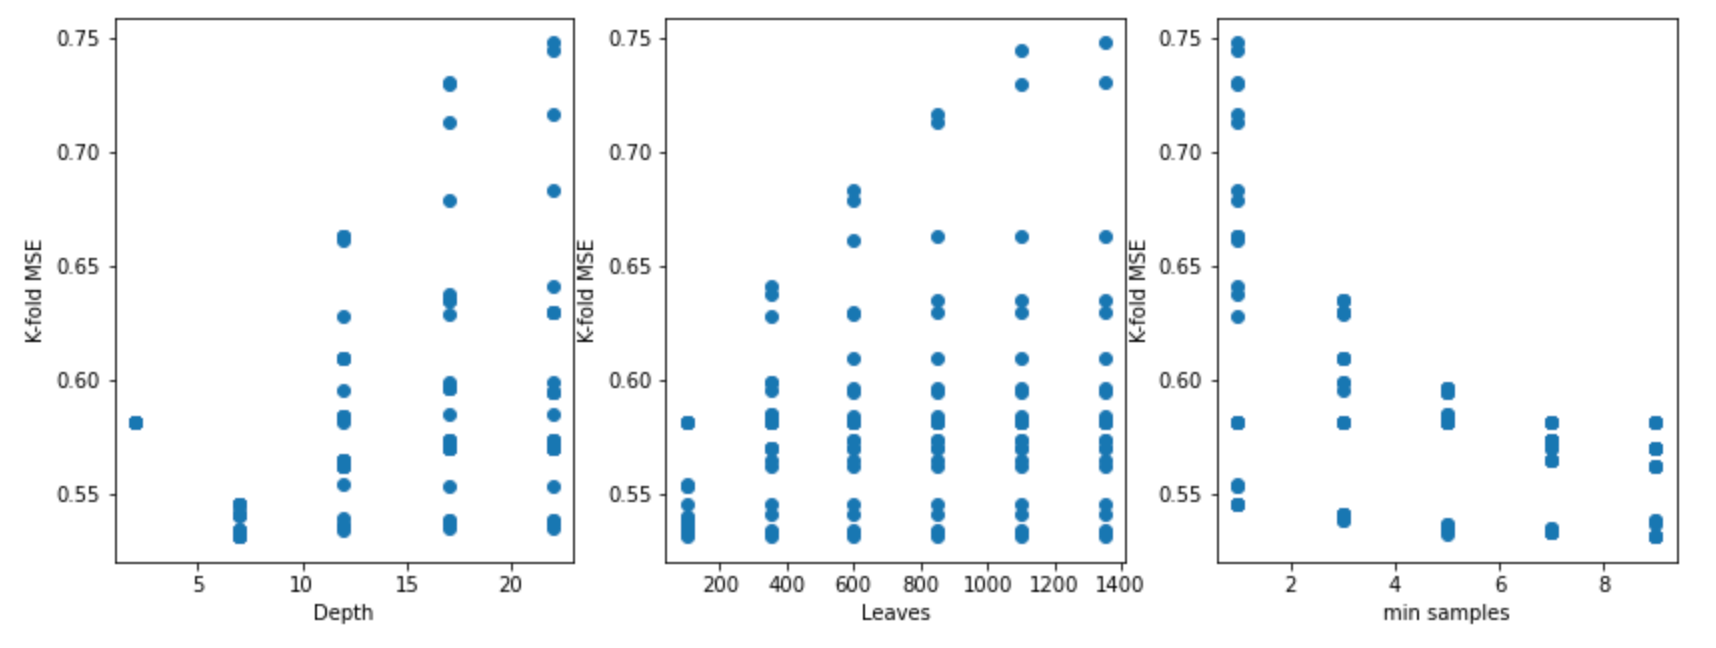
\includegraphics{Project_Report_Saturn_files/figure-pdf/tree1.png}

}

\caption{tree1.png}

\end{figure}

From this coarse grid search, I found that the best parameters were a
\texttt{max\_depth} of 7, \texttt{max\_leaf\_nodes} of 100, and
\texttt{min\_samples\_leaf} of 9. As some of these values were at the
end of the range of values I considered, I did a fine grid search. I
considered the following hyperparameter ranges:

\begin{Shaded}
\begin{Highlighting}[]
\CommentTok{\# Fine grid search parameters}
\NormalTok{fine\_grid }\OperatorTok{=}\NormalTok{ \{    }
    \StringTok{\textquotesingle{}max\_depth\textquotesingle{}}\NormalTok{: }\BuiltInTok{range}\NormalTok{(}\DecValTok{3}\NormalTok{,}\DecValTok{12}\NormalTok{),}
    \StringTok{\textquotesingle{}max\_leaf\_nodes\textquotesingle{}}\NormalTok{: np.arange(}\DecValTok{2}\NormalTok{, }\DecValTok{127}\NormalTok{, }\DecValTok{25}\NormalTok{),}
    \StringTok{\textquotesingle{}min\_samples\_leaf\textquotesingle{}}\NormalTok{: [}\DecValTok{8}\NormalTok{, }\DecValTok{9}\NormalTok{, }\DecValTok{10}\NormalTok{]}
\NormalTok{\}}
\end{Highlighting}
\end{Shaded}

\begin{figure}

{\centering 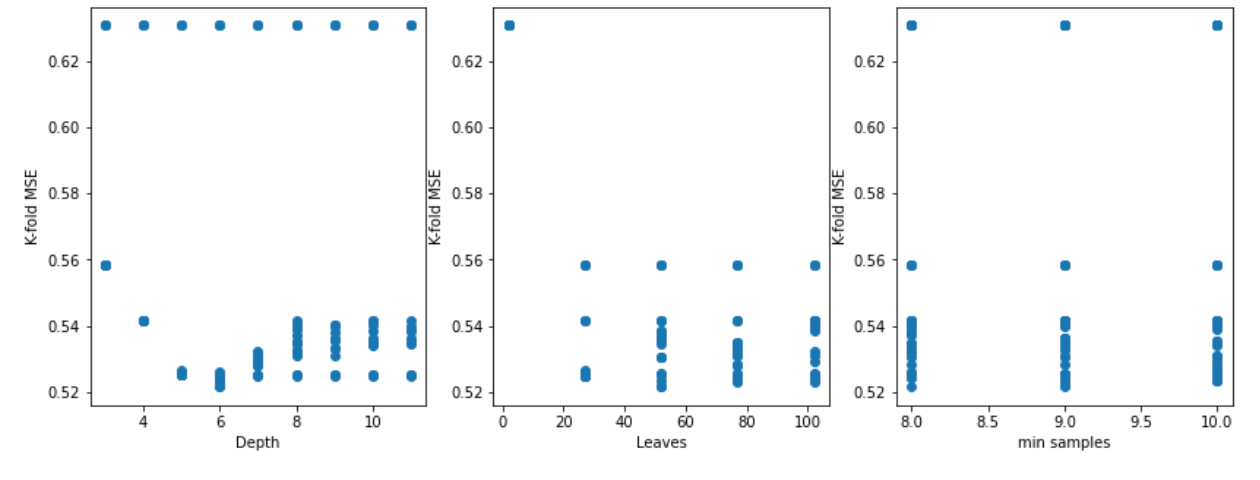
\includegraphics{Project_Report_Saturn_files/figure-pdf/tree2.png}

}

\caption{tree2.png}

\end{figure}

This \texttt{GridSearchCV()} gave optimal values of \texttt{max\_depth}
= 6, \texttt{max\_leaf\_nodes} = 52, and \texttt{min\_samples\_leaf} =
8. I trained a decision tree regressor using these optimal
hyperparameter values. Then, I used this model to predict the quality of
test data, rounding values to the closest integer. This gave me an RMSE
of 0.804.

\hypertarget{bagging-decision-trees}{%
\subsubsection{Bagging Decision Trees}\label{bagging-decision-trees}}

\emph{By Lila Wells}

I approached the bagging model in two phases (1) a coarse grid search to
identify the optimal hyperparameter space, and (2) a finer grid search
to optimize hyperparameters. Yet before both steps, I wanted to
determine (roughly) the number of trees that would be needed to
stabilize the model's R-squared and RMSE.

In the set of graphs below, I plotted the number of trees versus the out
of bag RMSE and test RMSE (\textbf{See Appendix A.2, Figure A.2.1}). I
noted that, while the test and out-of-bag R-squard trendlines seem to
intersect and start to stabilize after the number of trees exceeds
\textasciitilde400, the out-of-bag and test RMSE trendlines seem to
stabilize a little later, after around 500 trees. Thus, I chose 500 as
my lower bound for \texttt{n\_estimators} for the hyperparameter space.

\hypertarget{coarse-grid-search-1}{%
\paragraph{Coarse Grid Search}\label{coarse-grid-search-1}}

I elected to optimize the following parameters: (1) n\_estimators, (2)
max\_samples, (3) max\_feautres, (4) bootstrap, and (5) bootstrap
features. I considered the following ranges of hyperparamteters in my
initial coarse grid search:

\begin{Shaded}
\begin{Highlighting}[]
\CommentTok{\# Parameters for the coarse grid search}
\CommentTok{\textquotesingle{}estimator\textquotesingle{}}\NormalTok{: [DecisionTreeRegressor(random\_state }\OperatorTok{=} \DecValTok{1}\NormalTok{), DecisionTreeRegressor(random\_state }\OperatorTok{=} \DecValTok{1}\NormalTok{, max\_depth }\OperatorTok{=} \DecValTok{6}\NormalTok{), DecisionTreeRegressor(random\_state }\OperatorTok{=} \DecValTok{1}\NormalTok{, max\_depth }\OperatorTok{=} \DecValTok{10}\NormalTok{)],}
\CommentTok{\textquotesingle{}n\_estimators\textquotesingle{}}\NormalTok{: }\BuiltInTok{range}\NormalTok{(}\DecValTok{500}\NormalTok{, }\DecValTok{1001}\NormalTok{, }\DecValTok{100}\NormalTok{),}
\CommentTok{\textquotesingle{}max\_samples\textquotesingle{}}\NormalTok{: [}\FloatTok{0.5}\NormalTok{, }\FloatTok{0.75}\NormalTok{, }\FloatTok{1.0}\NormalTok{],}
\CommentTok{\textquotesingle{}max\_features\textquotesingle{}}\NormalTok{: [}\FloatTok{0.5}\NormalTok{, }\FloatTok{1.0}\NormalTok{],}
\CommentTok{\textquotesingle{}bootstrap\textquotesingle{}}\NormalTok{: [}\VariableTok{True}\NormalTok{, }\VariableTok{False}\NormalTok{],}
\CommentTok{\textquotesingle{}bootstrap\_features\textquotesingle{}}\NormalTok{: [}\VariableTok{True}\NormalTok{, }\VariableTok{False}\NormalTok{]\}}
\end{Highlighting}
\end{Shaded}

I considered three different types of decision trees. The first was a
base decision tree with \texttt{random\_state\ =\ 1} and no specified
\texttt{max\_depth} or other hyperparameters. The second tree had a
\texttt{max\_depth} of 6 (the optimal value found in Kaitlyn's decision
tree optimization process. I included that tree to test whether
specifying \texttt{max\_depth} could have a beneficial impact on the
model's RMSE. The final tree had a \texttt{max\_depth} of 10, and was
included as a way to test whether specifying an additional
hyperparameter could yield postiive results in the search process.

I then used the above parameters as a grid to iterate through using
\texttt{GridSearchCV()} and 2 fold cross-validation (to minimize runtime
and identify the range of hyperparameters to focus in on in my finer
grid search).

This coarse grid search identified the following optimal
hyperparameters: (1) \texttt{estimator}:
DecisionTreeRegressor(random\_state = 1), (2) \texttt{n\_estimators}:
1000, (3) \texttt{max\_samples}: 0.75, (4)\texttt{max\_features}: 1.0,
(5) \texttt{bootstrap}: False, (6) \texttt{bootstrap\_features}: True

With these hyperparameters, the model yielded a 0.667 test RMSE. I
graphed and inspected the results of the \texttt{GridSearchCV()} search
with 2-fold cross validation to identify which distributions I should
inspect for my finer grid search (in an effort to reduce the model's
RMSE). (\textbf{See Appendix A.2. Figure A.2.2}).

\hypertarget{finer-grid-search}{%
\paragraph{Finer Grid Search}\label{finer-grid-search}}

Based on the above graphs and the optimal hyperparameters identified in
my coarse grid search, I altered my hyperparameter distribution for the
finer grid search as follows:

\begin{Shaded}
\begin{Highlighting}[]
\CommentTok{\textquotesingle{}estimator\textquotesingle{}}\NormalTok{: [DecisionTreeRegressor(random\_state }\OperatorTok{=} \DecValTok{1}\NormalTok{)], }\CommentTok{\# Narrowing this search space baesed on coarse grid results}
\CommentTok{\textquotesingle{}n\_estimators\textquotesingle{}}\NormalTok{: }\BuiltInTok{range}\NormalTok{(}\DecValTok{800}\NormalTok{, }\DecValTok{1101}\NormalTok{, }\DecValTok{60}\NormalTok{),, }\CommentTok{\# Narrowing this search space based on coarse grid results}
\CommentTok{\textquotesingle{}max\_samples\textquotesingle{}}\NormalTok{: [}\FloatTok{0.6}\NormalTok{, }\FloatTok{0.75}\NormalTok{, }\FloatTok{0.9}\NormalTok{], }\CommentTok{\# Narrowing this search space based on coarse grid results}
\CommentTok{\textquotesingle{}max\_features\textquotesingle{}}\NormalTok{: [}\FloatTok{0.5}\NormalTok{, }\FloatTok{0.75}\NormalTok{, }\FloatTok{0.85}\NormalTok{, }\FloatTok{1.0}\NormalTok{] }\CommentTok{\# Narrowing this search space based on coarse grid results}
\CommentTok{\textquotesingle{}bootstrap\textquotesingle{}}\NormalTok{: [}\VariableTok{True}\NormalTok{, }\VariableTok{False}\NormalTok{],}
\CommentTok{\textquotesingle{}bootstrap\_features\textquotesingle{}}\NormalTok{: [}\VariableTok{True}\NormalTok{, }\VariableTok{False}\NormalTok{]\}}
\end{Highlighting}
\end{Shaded}

I then used the above parameters as a grid to iterate through using
\texttt{GridSearchCV()} and 2 fold cross-validation (to minimize runtime
and identify the range of hyperparameters to focus in on in my finer
grid search).

This coarse grid search identified the following optimal
hyperparameters: (1)\texttt{estimator}:
DecisionTreeRegressor(random\_state = 1), (2) \texttt{n\_estimators}:
1040, (3) \texttt{max\_samples}: 0.75, (4) \texttt{max\_features}: 0.75,
(5) \texttt{bootstrap1:\ False,\ (6)}bootstrap\_features`: False

With these hyperparameters, the model yielded a 0.665 test RMSE, a
slight improvement from my original RMSE of 0.667. I graphed and
inspected the results of the \texttt{GridSearchCV()} search with 2-fold
cross validation to better inspect the distributions of my
hyperparameter values (\textbf{See Appendix A.2. Figure A.2.3}).

I attempted several more grid searches with different values for
\texttt{n\_estimators} (as my optimal \texttt{n\_estimators} value of
1040 was at the upper range of that hyperparameter space in the fine
grid search). However, the test RMSE of my model did not improve. Thus,
this fine grid search yielded the optimal hyperparameters for this
model.

\hypertarget{random-forest}{%
\subsubsection{Random Forest}\label{random-forest}}

\emph{By Amy Wang}

I start by conducting a GridSearchCV to determine the optimal number of
\texttt{max\_features}, and find that 3 features is optimal.
\textgreater{} \texttt{max\_features}: range(1, 14, 1)

I then manually create a few different models with 3 features and
varying numbers of \texttt{n\_estimators}. I find that 4000 estimators
gave the lowest test RMSE. \textgreater{} 900 estimators:
0.6725382459813659 \textgreater{} 4000 estimators: 0.6592536572635639
\textgreater{} 6000 estimators: 0.6604194471348085

I next try holding \texttt{max\_features\ =\ 3} and
\texttt{n\_estimators\ =\ 4000} constant, while tuning for
\texttt{max\_depth} and \texttt{max\_samples}.

\begin{quote}
params = \{`n\_estimators': {[}4000{]}, `max\_features': range(1, 14,
2), `max\_depth': {[}3{]}, `max\_samples': range(1,
X\_train.shape{[}0{]}, 500)\}
\end{quote}

The optimal combination of parameters returned by RandomizedSearchCV
\texttt{\{\textquotesingle{}n\_estimators\textquotesingle{}:\ 4000,\ \textquotesingle{}max\_samples\textquotesingle{}:\ 501,\ \textquotesingle{}max\_features\textquotesingle{}:\ 9,\ \textquotesingle{}max\_depth\textquotesingle{}:\ 3\}}
gave an RMSE that was significantly higher than my base RMSE:
0.7975925314055079.

I decide to then attempt to tune all four parameters simultaneously with
RandomizedSearchCV.

\begin{quote}
params = \{`n\_estimators': range(100, 5000, 100), `max\_features':
range(1, 14, 2), `max\_depth': range(2,30, 2), `max\_samples': range(1,
X\_train.shape{[}0{]}, 500)\}
\end{quote}

The optimal combination of parameters was
\texttt{\{\textquotesingle{}n\_estimators\textquotesingle{}:\ 1700,\ \textquotesingle{}max\_samples\textquotesingle{}:\ 4001,\ \textquotesingle{}max\_features\textquotesingle{}:\ 7,\ \textquotesingle{}max\_depth\textquotesingle{}:\ 20\}},
which gave a test RMSE of 0.6821910402406465. This was higher than the
\texttt{\{\textquotesingle{}n\_estimators\textquotesingle{}:\ 4000,\ \textquotesingle{}max\_features\textquotesingle{}:\ 3\}}
model's RMSE, so I manually increase \texttt{n\_estimators} and tune
\texttt{max\_depth} based on the decreasing trend in the plot.

\begin{quote}
\{`n\_estimators': 3700, `max\_samples': 5000, `max\_features': 7,
`max\_depth': 20\} - Test RMSE 0.6713934992009014 \{`n\_estimators':
5000, `max\_samples': 5000, `max\_features': 7, `max\_depth': 35\} -
Test RMSE 0.6702467972551374 \{`n\_estimators': 4000, `max\_samples':
5000, `max\_features': 7, `max\_depth': 50\} - Test RMSE
0.6690981300917733
\end{quote}

Overall, the best random forest model was
\texttt{\{\textquotesingle{}n\_estimators\textquotesingle{}:\ 4000,\ \textquotesingle{}max\_features\textquotesingle{}:\ 3\}},
which had an RMSE of 0.6592536572635639.

\hypertarget{adaboost}{%
\subsubsection{AdaBoost}\label{adaboost}}

\emph{By Kaitlyn Hung}

I optimized the following hyperparameters: \texttt{n\_estimators},
\texttt{learning\_rate}, and \texttt{max\_depth} of the base estimator
using \texttt{GridSearchCV()} to identify the optimal hyperparameter
values. In my coarse grid search, I considered the following ranges:

\begin{Shaded}
\begin{Highlighting}[]
\CommentTok{\# Coarse grid search parameters considered}
\NormalTok{grid[}\StringTok{\textquotesingle{}n\_estimators\textquotesingle{}}\NormalTok{] }\OperatorTok{=}\NormalTok{ [}\DecValTok{10}\NormalTok{, }\DecValTok{50}\NormalTok{, }\DecValTok{100}\NormalTok{,}\DecValTok{200}\NormalTok{]}
\NormalTok{grid[}\StringTok{\textquotesingle{}learning\_rate\textquotesingle{}}\NormalTok{] }\OperatorTok{=}\NormalTok{ [}\FloatTok{0.0001}\NormalTok{, }\FloatTok{0.001}\NormalTok{, }\FloatTok{0.01}\NormalTok{,}\FloatTok{0.1}\NormalTok{, }\FloatTok{1.0}\NormalTok{]}
\NormalTok{grid[}\StringTok{\textquotesingle{}base\_estimator\_\_max\_depth\textquotesingle{}}\NormalTok{] }\OperatorTok{=}\NormalTok{ [}\DecValTok{3}\NormalTok{, }\DecValTok{5}\NormalTok{, }\DecValTok{10}\NormalTok{, }\DecValTok{15}\NormalTok{]}
\end{Highlighting}
\end{Shaded}

This gave the optimal hyperparameters to be a \texttt{max\_depth} of 15,
\texttt{n\_estimators} as 200, and \texttt{learning\_rate} as 1 (See
appendix A4 for the relevant figure). These were the max values I
considered for each of the hyperparameters, so I did another grid
search, increasing the values I considered (Refer to appendix A4 for the
next two grid searches). After performing two more grid searches, the
optimal values of some of the hyperaprameters were at the end of of the
range, so I increased the values I considered. I tuned
\texttt{max\_depth} and \texttt{learning\_rate} separately from
\texttt{n\_estimators} as thus far, the highest value of
\texttt{n\_estimators} has been best.

\begin{Shaded}
\begin{Highlighting}[]
\CommentTok{\# Learning rate and max depths considered}
\NormalTok{grid[}\StringTok{\textquotesingle{}learning\_rate\textquotesingle{}}\NormalTok{] }\OperatorTok{=}\NormalTok{ [}\FloatTok{1.25}\NormalTok{, }\FloatTok{1.5}\NormalTok{, }\DecValTok{2}\NormalTok{]}
\NormalTok{grid[}\StringTok{\textquotesingle{}base\_estimator\_\_max\_depth\textquotesingle{}}\NormalTok{] }\OperatorTok{=}\NormalTok{ [}\DecValTok{12}\NormalTok{, }\DecValTok{13}\NormalTok{, }\DecValTok{14}\NormalTok{]}
\end{Highlighting}
\end{Shaded}

\begin{figure}

{\centering 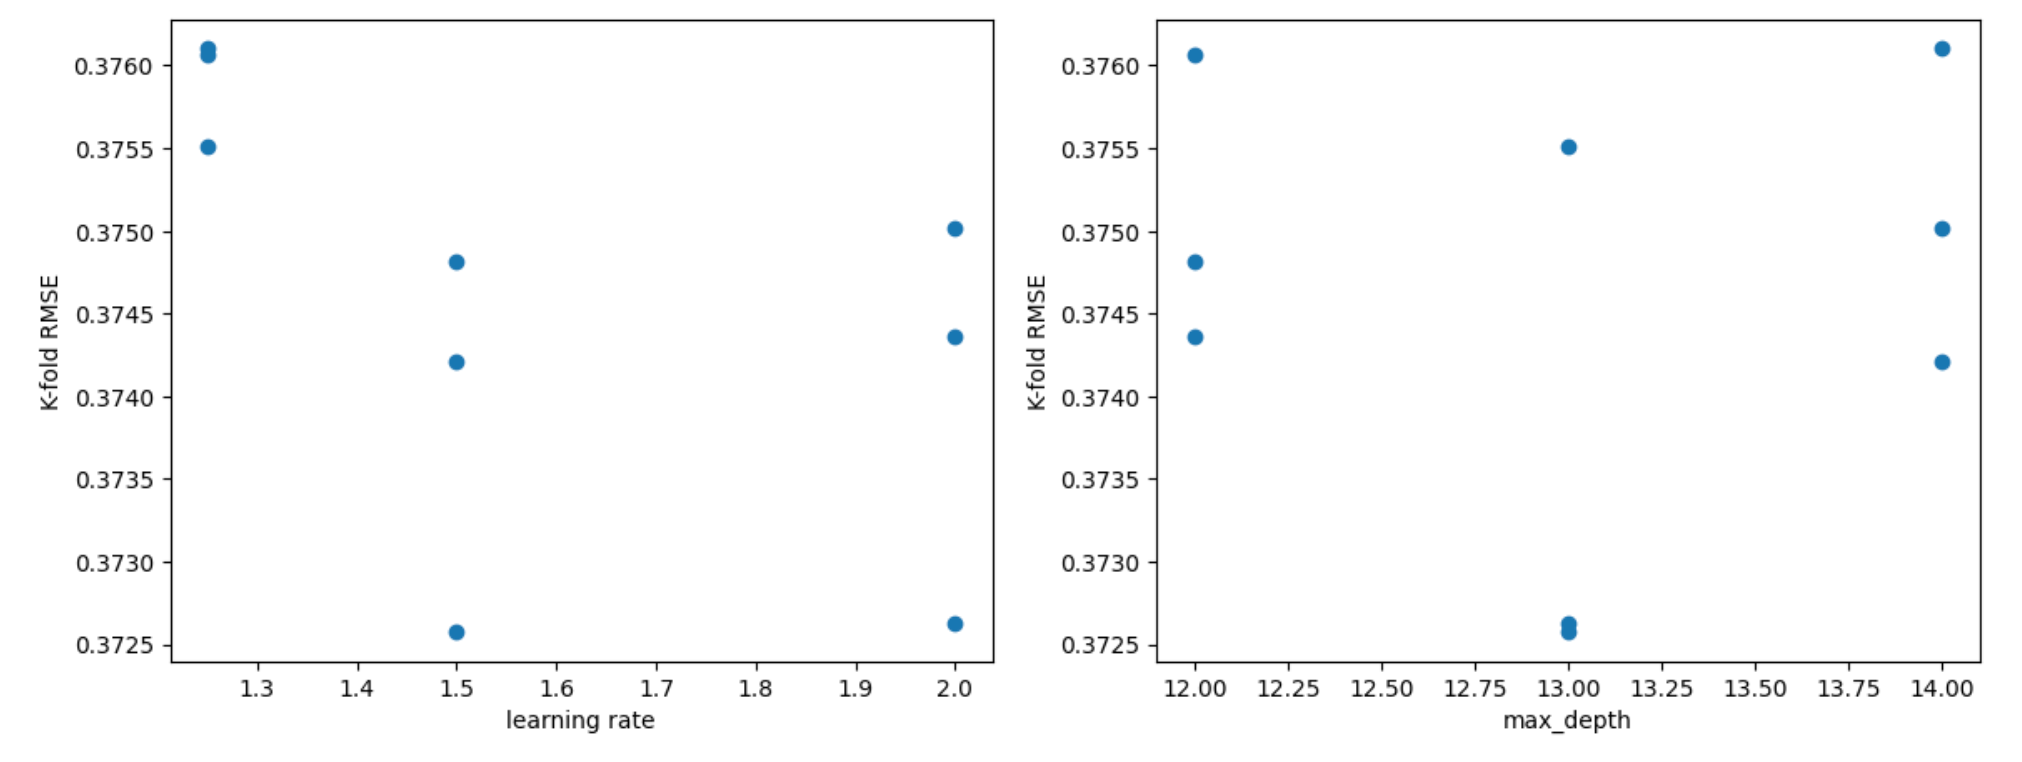
\includegraphics{Project_Report_Saturn_files/figure-pdf/ada4.png}

}

\caption{ada4.png}

\end{figure}

I found that a \texttt{max\_depth} of 13 and \texttt{learning\_rate} of
1.5 still gave the lowest RMSE. Using these optimal values, I next tuned
\texttt{n\_estimators}, considering the following values:

\begin{Shaded}
\begin{Highlighting}[]
\CommentTok{\# N\_estimators values considered}
\NormalTok{grid[}\StringTok{\textquotesingle{}n\_estimators\textquotesingle{}}\NormalTok{] }\OperatorTok{=}\NormalTok{ [}\DecValTok{1000}\NormalTok{, }\DecValTok{1500}\NormalTok{, }\DecValTok{2000}\NormalTok{, }\DecValTok{3000}\NormalTok{, }\DecValTok{4000}\NormalTok{]}
\end{Highlighting}
\end{Shaded}

Using \texttt{n\_estimators} equal to 2000 appeared to be best. However,
when I calculated the RMSE using n\_estimators as 1500 and 2000, I found
that 1500 actually gave the lowest RMSE. I created an
\texttt{AdaBoostRegressor} model using n\_estimators as 1500,
\texttt{max\_depth} as 13, and learning\_rate as 1.5, rounded the
predictions to the nearest integer, and found that this model had an
RMSE of 0.658.

\hypertarget{gradient-boosting}{%
\subsubsection{Gradient Boosting}\label{gradient-boosting}}

\emph{By Anastasia Wei}

I used the \texttt{GradientBoostingRegressor} from the
\texttt{sklearn.ensemble} modulo with the huber loss function for the
model. First I used 5 fold cross validation to get a sense of the number
of estimators I need to reach a stable cross validation RMSE and found
that around 1500 trees will be sufficient.

\begin{figure}

{\centering 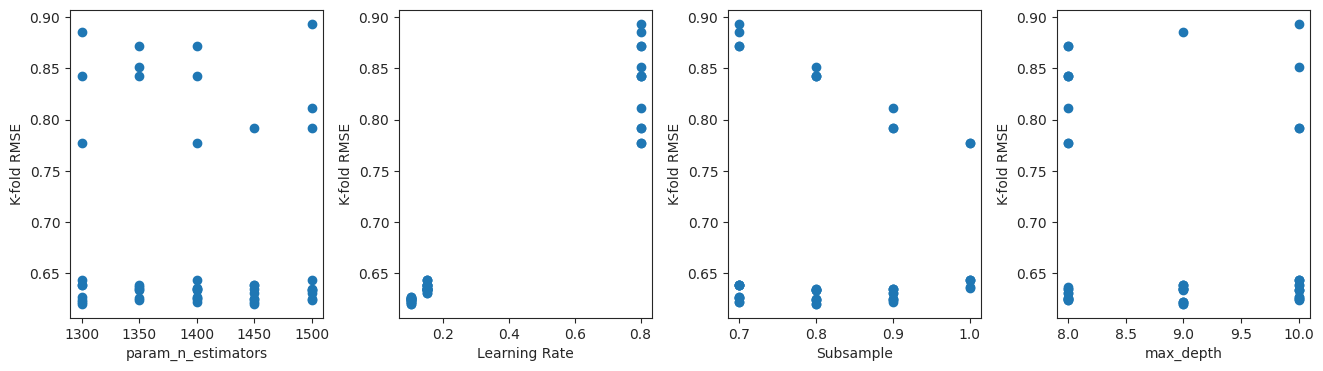
\includegraphics{Project_Report_Saturn_files/figure-pdf/image.png}

}

\caption{image.png}

\end{figure}

With this information, I started with a coarse grid search with 4 fold
cross validation (to speed up the training process) using
\texttt{RandomizedSearchCV} with 50 iterations.

\begin{Shaded}
\begin{Highlighting}[]
\CommentTok{\# Parameter grid for gradient boosting model coarse grid search}
\NormalTok{grid[}\StringTok{\textquotesingle{}n\_estimators\textquotesingle{}}\NormalTok{] }\OperatorTok{=}\NormalTok{ [}\DecValTok{1200}\NormalTok{, }\DecValTok{1400}\NormalTok{, }\DecValTok{1600}\NormalTok{, }\DecValTok{1800}\NormalTok{]}
\NormalTok{grid[}\StringTok{\textquotesingle{}learning\_rate\textquotesingle{}}\NormalTok{] }\OperatorTok{=}\NormalTok{ [}\FloatTok{0.1}\NormalTok{, }\FloatTok{0.2}\NormalTok{, }\FloatTok{0.3}\NormalTok{]}
\NormalTok{grid[}\StringTok{\textquotesingle{}max\_depth\textquotesingle{}}\NormalTok{] }\OperatorTok{=}\NormalTok{ [}\DecValTok{8}\NormalTok{, }\DecValTok{10}\NormalTok{, }\DecValTok{12}\NormalTok{, }\DecValTok{14}\NormalTok{]}
\NormalTok{grid[}\StringTok{\textquotesingle{}subsample\textquotesingle{}}\NormalTok{] }\OperatorTok{=}\NormalTok{ [}\FloatTok{0.4}\NormalTok{, }\FloatTok{0.6}\NormalTok{, }\FloatTok{0.8}\NormalTok{, }\DecValTok{1}\NormalTok{]}
\end{Highlighting}
\end{Shaded}

I found a best cross validation RMSE of 0.6237 using
\texttt{\textquotesingle{}subsample\textquotesingle{}:\ 0.8,\ \textquotesingle{}n\_estimators\textquotesingle{}:\ 1400,\ \textquotesingle{}max\_depth\textquotesingle{}:\ 8,\ \textquotesingle{}learning\_rate\textquotesingle{}:\ 0.1}
and test RMSE of 0.6777. I visualized the parameters as follows:

\begin{figure}

{\centering 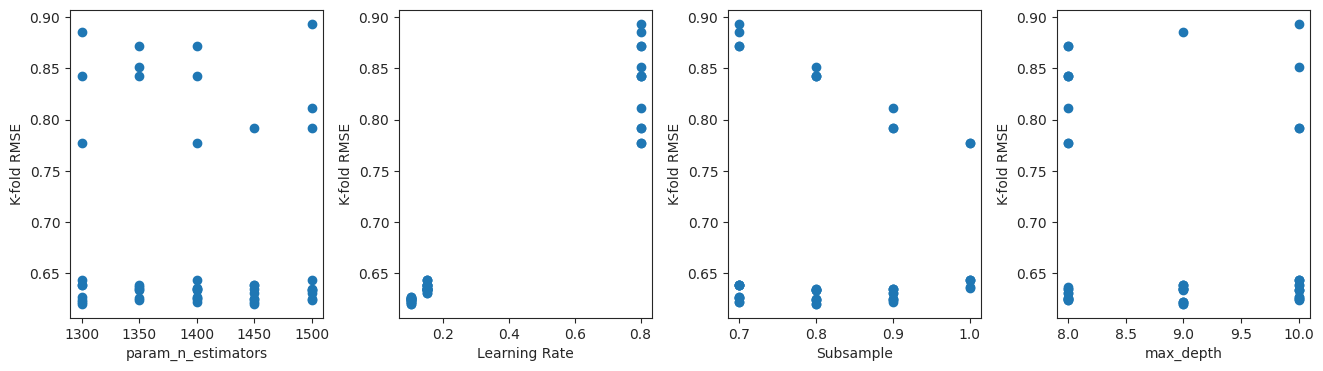
\includegraphics{Project_Report_Saturn_files/figure-pdf/image.png}

}

\caption{image.png}

\end{figure}

Then I implemented a finer tunning zooming in on the parameter space
with the lowest k-fold RMSE. The search grid is as follows:

\begin{Shaded}
\begin{Highlighting}[]
\CommentTok{\# Parameter grid for gradient boosting model fine grid search}
\NormalTok{grid[}\StringTok{\textquotesingle{}n\_estimators\textquotesingle{}}\NormalTok{] }\OperatorTok{=}\NormalTok{ [}\DecValTok{1300}\NormalTok{, }\DecValTok{1350}\NormalTok{, }\DecValTok{1400}\NormalTok{, }\DecValTok{1450}\NormalTok{, }\DecValTok{1500}\NormalTok{]}
\NormalTok{grid[}\StringTok{\textquotesingle{}learning\_rate\textquotesingle{}}\NormalTok{] }\OperatorTok{=}\NormalTok{ [}\FloatTok{0.8}\NormalTok{, }\FloatTok{0.1}\NormalTok{, }\FloatTok{0.15}\NormalTok{]}
\NormalTok{grid[}\StringTok{\textquotesingle{}max\_depth\textquotesingle{}}\NormalTok{] }\OperatorTok{=}\NormalTok{ [}\DecValTok{8}\NormalTok{, }\DecValTok{9}\NormalTok{, }\DecValTok{10}\NormalTok{]}
\NormalTok{grid[}\StringTok{\textquotesingle{}subsample\textquotesingle{}}\NormalTok{] }\OperatorTok{=}\NormalTok{ [}\FloatTok{0.7}\NormalTok{, }\FloatTok{0.8}\NormalTok{, }\FloatTok{0.9}\NormalTok{, }\DecValTok{1}\NormalTok{]}
\end{Highlighting}
\end{Shaded}

I found a best cross validation RMSE of 0.6204 using
\texttt{\textquotesingle{}subsample\textquotesingle{}:\ 0.8,\ \textquotesingle{}n\_estimators\textquotesingle{}:\ 1300,\ \textquotesingle{}max\_depth\textquotesingle{}:\ 9,\ \textquotesingle{}learning\_rate\textquotesingle{}:\ 0.1}
and test RMSE of 0.6713. I visualized the parameters as follows:
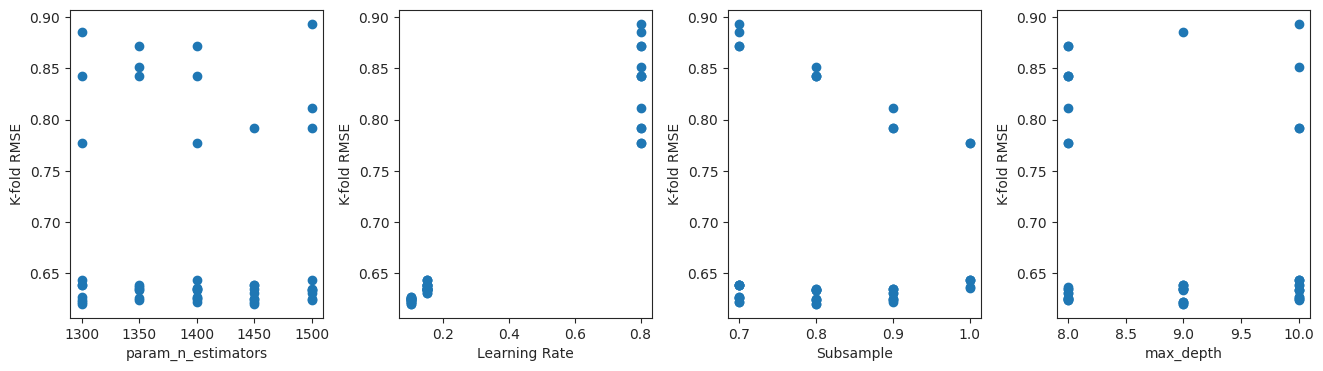
\includegraphics{Project_Report_Saturn_files/figure-pdf/image.png}

After this fine tuning, I did some manual tuning by making minor changes
to the optimal parameters and combinations of parameters that are
correlated (e.g.~n\_estimators and learning\_rate) given by this tuning.
However, the performance of the model did not change significantly. The
only changed the improved the model significantly was increasing the
subsample rate from 0.8 to 0.85. This resulted in a test RMSE of 0.6587.

\hypertarget{xgboost}{%
\subsubsection{XGBoost}\label{xgboost}}

\emph{By Amy Wang}

To tune an XGBoost model for the Vinho Verde dataset, I first conduct a
broad sweep of the parameter space with \texttt{RandomizedSearchCV} with
the following grid:

\begin{quote}
param\_grid = \{`max\_depth': {[}4, 5, 6, 7, 8, 9{]}, `learning\_rate':
{[}0.01{]}, `reg\_lambda':{[}0, 10, 20, 30, 40, 70, 100{]},
`n\_estimators':{[}3000, 4000, 5000{]}, `gamma': {[}0, 3, 5, 7, 10{]},
`subsample': {[}0.5, 1.0{]}, ``colsample\_bytree'': {[}0.6, 0.75, 0.8,
0.9{]}\}
\end{quote}

I obtain this combination of optimal parameters
\texttt{\{\textquotesingle{}subsample\textquotesingle{}:\ 1.0,\ \textquotesingle{}reg\_lambda\textquotesingle{}:\ 0,\ \textquotesingle{}n\_estimators\textquotesingle{}:\ 2000,\ \textquotesingle{}max\_depth\textquotesingle{}:\ 8,\ \textquotesingle{}learning\_rate\textquotesingle{}:\ 0.01,\ \textquotesingle{}gamma\textquotesingle{}:\ 0,\ \textquotesingle{}colsample\_bytree\textquotesingle{}:\ 1.0\}}.
An XGBoost model fit with these parameters predicted the test data with
an RMSE of 0.6799.

I visualize the plots of each parameter against the 5-fold
cross-validated RMSE in attempt to manually tune the parameters
(Appendix A6, Figure 1). Changing the parameters to
\texttt{\{n\_estimators\ =\ 4000,\ learning\_rate\ =\ 0.01,\ subsample\ =\ 1.0,\ reg\_lambda\ =\ 100,\ max\_depth\ =\ 8,\ gamma\ =\ 0,\ colsample\_bytree\ =\ 1.0\}}
based on the trends in the plots gave a higher RMSE of 0.6856.

The only clear insight gained from the plots was that the optimal
learning rate is 0.01. I then conducted a second
\texttt{RandomizedSearchCV} with a fixed learning rate of 0.01 and
spanning a range of the other 6 variables. I used the following grid
with 50 iterations:

\begin{quote}
param\_grid = \{`max\_depth': {[}4, 5, 6, 7, 8, 9{]}, `learning\_rate':
{[}0.01{]}, `reg\_lambda':{[}0, 10, 20, 30, 40, 70, 100{]},
`n\_estimators':{[}3000, 4000, 5000{]}, `gamma': {[}0, 3, 5, 7, 10{]},
`subsample': {[}0.5, 1.0{]}, `colsample\_bytree': {[}0.6, 0.75, 0.8,
0.9{]}\}
\end{quote}

The optimal parameters obtained from this second search were
\texttt{\{\textquotesingle{}subsample\textquotesingle{}:\ 0.5,\ \textquotesingle{}reg\_lambda\textquotesingle{}:\ 0,\ \textquotesingle{}n\_estimators\textquotesingle{}:\ 5000,\ \textquotesingle{}max\_depth\textquotesingle{}:\ 9,\ \textquotesingle{}learning\_rate\textquotesingle{}:\ 0.01,\ \textquotesingle{}gamma\textquotesingle{}:\ 0,\ \textquotesingle{}colsample\_bytree\textquotesingle{}:\ 0.75\}}.
A model fit with the optimal parameters from the second search gave an
RMSE of 0.6598. Plotting the parameters against a 5-fold cross-validated
RMSE showed that each parameter was already at its most optimal.

I explore hyperparameter tuning with Bayesian Optimization in attempt to
lower the RMSE further (Appendix A6, Method 1). RandomizedSearchCV tests
a random combination of the parameters in the grid, and therefore may
have missed certain areas of the parameter space. Bayesian Optimization
balances searching new areas of the parameter space with hyperfocusing
on tuning the optimal parameters from optimal regions of the space. This
method gave a higher RMSE than my best with RandomizedSearchCV, so I
move forward with RandomizedSearchCV parameters.

\hypertarget{catboost-and-lightgbm}{%
\subsubsection{CatBoost, and LightGBM}\label{catboost-and-lightgbm}}

\emph{By Anastasia Wei}

I fit the data with \texttt{CatBoostRegressor} model from the
\texttt{catboost} package using the default parameters and it gave a
train RMSE of 0.4761 and a test RMSE of 0.7131. Then I also fit the data
with a \texttt{LGBMRegressor} model from the \texttt{lightbm} package
using the default parameters. It yielded a train RMSE of 0.5211 and a
test RMSE of 0.7259.

We decided to include CatBoost and LightGBM models to (1) increase the
diversity of the ensemble models and (2) see whether they will perform
better than our other base models. However, these two models are
additional base models and were included more for experimentation than
the purpose of rigorous optimization (thus, we did not continue to
optimize the CatBoost and LightGBM hyperparameters beyond their
defaults).

\hypertarget{model-ensemble}{%
\subsection{Model Ensemble}\label{model-ensemble}}

\hypertarget{voting-ensemble}{%
\subsubsection{Voting ensemble}\label{voting-ensemble}}

\emph{By Anastasia Wei}

I used the \texttt{VotingRegressor} from \texttt{sklearn.ensemble} to
create the voting ensemble model. I chose to only use the XGBoost,
AdaBoost, Random Rorest, Gradient Boost, and Bagging Models in this
ensemble as the other base models (CatBoost, LightGBM, Lasso, Ridge,
MARS) had higher test RMSEs (\textgreater{} 0.7).

The voting ensemble model yielded a test RMSE of 0.651 (lower than each
of the individual models). (\emph{See below for a plot of the actual vs
predicted response}).

\hypertarget{stacking-ensemble}{%
\subsubsection{Stacking ensemble}\label{stacking-ensemble}}

\emph{By Anastasia Wei}

I first fit each of the models mentioned about on the train and test
dataset to create a new test and train datasets to fit the metamodels
on. See the following subsections for the individual metamodels.

\hypertarget{linear-regression-metamodel}{%
\paragraph{Linear Regression
Metamodel}\label{linear-regression-metamodel}}

Using \texttt{LinearRegression} from \texttt{sklearn.LinearModels} on
the new train data set, I obtained a test RMSE of 0.6714.

\hypertarget{lasso-metamodel}{%
\paragraph{Lasso Metamodel}\label{lasso-metamodel}}

Using regularization parameter alphas in the range of
\texttt{10**np.linspace(0,\ -3,\ 300)*0.5}, I tuned the model using
LassoCV. With the optimal alpha of 0.0005, I obtained a test RMSE of
0.6598.

\hypertarget{mars-metamodel}{%
\paragraph{MARS Metamodel}\label{mars-metamodel}}

I fit a MARS model using \texttt{Earth} from \texttt{pyearth} package
with degree 1 to avoid overfitting. This gave a test RMSE of 0.6593.

\hypertarget{random-forest-metamodel}{%
\paragraph{Random Forest Metamodel}\label{random-forest-metamodel}}

I tuned a random forest metamodel using the following parameter space
with 4 fold cross validation with \texttt{RandomizedSearchCV} using 100
iterations.

\begin{Shaded}
\begin{Highlighting}[]
\CommentTok{\# Parameter grid for Random Forest metamodel}
\NormalTok{param\_grid }\OperatorTok{=}\NormalTok{ \{}\StringTok{\textquotesingle{}n\_estimators\textquotesingle{}}\NormalTok{: [}\DecValTok{100}\NormalTok{],}
              \StringTok{\textquotesingle{}max\_depth\textquotesingle{}}\NormalTok{: [}\DecValTok{8}\NormalTok{, }\DecValTok{10}\NormalTok{, }\DecValTok{12}\NormalTok{, }\DecValTok{14}\NormalTok{],}
              \StringTok{\textquotesingle{}max\_leaf\_nodes\textquotesingle{}}\NormalTok{:[}\DecValTok{100}\NormalTok{, }\DecValTok{500}\NormalTok{, }\DecValTok{1000}\NormalTok{],}
              \StringTok{\textquotesingle{}max\_features\textquotesingle{}}\NormalTok{: [}\DecValTok{2}\NormalTok{, }\DecValTok{4}\NormalTok{, }\DecValTok{6}\NormalTok{, }\DecValTok{8}\NormalTok{],}
              \StringTok{\textquotesingle{}max\_samples\textquotesingle{}}\NormalTok{: [}\DecValTok{1000}\NormalTok{, }\DecValTok{2000}\NormalTok{, }\DecValTok{3000}\NormalTok{]\}}
\end{Highlighting}
\end{Shaded}

This search yielded the following optimal parameters:
\texttt{\textquotesingle{}n\_estimators\textquotesingle{}:\ 100,\ \textquotesingle{}max\_samples\textquotesingle{}:\ 3000,\ \textquotesingle{}max\_leaf\_nodes\textquotesingle{}:\ 1000,\ \textquotesingle{}max\_features\textquotesingle{}:\ 8,\ \textquotesingle{}max\_depth\textquotesingle{}:\ 12}.
The test RMSE is 0.6482 using these optimal parameters.

\hypertarget{xgboost-metamodel}{%
\paragraph{XGBoost Metamodel}\label{xgboost-metamodel}}

I tuned a xgboost metamodel using the following parameter space with 4
fold cross validation with \texttt{RandomizedSearchCV} using 100
iterations. The parameter grid for this metamodel is detailed below:

\begin{Shaded}
\begin{Highlighting}[]
\CommentTok{\# Parameter grid for the XGBoost metamodel}
\NormalTok{param\_grid }\OperatorTok{=}\NormalTok{ \{}\StringTok{\textquotesingle{}max\_depth\textquotesingle{}}\NormalTok{: [}\DecValTok{3}\NormalTok{, }\DecValTok{4}\NormalTok{, }\DecValTok{5}\NormalTok{, }\DecValTok{6}\NormalTok{],}
              \StringTok{\textquotesingle{}learning\_rate\textquotesingle{}}\NormalTok{: [}\FloatTok{0.008}\NormalTok{, }\FloatTok{0.01}\NormalTok{, }\FloatTok{0.025}\NormalTok{, }\FloatTok{0.05}\NormalTok{],}
              \StringTok{\textquotesingle{}reg\_lambda\textquotesingle{}}\NormalTok{:[}\DecValTok{0}\NormalTok{, }\DecValTok{1}\NormalTok{, }\DecValTok{5}\NormalTok{],}
              \StringTok{\textquotesingle{}n\_estimators\textquotesingle{}}\NormalTok{:[}\DecValTok{500}\NormalTok{, }\DecValTok{600}\NormalTok{, }\DecValTok{800}\NormalTok{, }\DecValTok{1000}\NormalTok{],}
              \StringTok{\textquotesingle{}gamma\textquotesingle{}}\NormalTok{: [}\DecValTok{0}\NormalTok{, }\DecValTok{3}\NormalTok{, }\DecValTok{5}\NormalTok{, }\DecValTok{10}\NormalTok{],}
              \StringTok{\textquotesingle{}subsample\textquotesingle{}}\NormalTok{: [}\FloatTok{0.5}\NormalTok{, }\FloatTok{0.75}\NormalTok{, }\FloatTok{1.0}\NormalTok{],}
              \StringTok{\textquotesingle{}colsample\_bytree\textquotesingle{}}\NormalTok{: [}\FloatTok{0.5}\NormalTok{, }\FloatTok{0.75}\NormalTok{, }\FloatTok{1.0}\NormalTok{]\}}
\end{Highlighting}
\end{Shaded}

This search yielded the following optimal parameters:
\texttt{\textquotesingle{}subsample\textquotesingle{}:\ 0.75,\ \textquotesingle{}reg\_lambda\textquotesingle{}:\ 0,\ \textquotesingle{}n\_estimators\textquotesingle{}:\ 1000,\ \textquotesingle{}max\_depth\textquotesingle{}:\ 6,\ \textquotesingle{}learning\_rate\textquotesingle{}:\ 0.008,\ \textquotesingle{}gamma\textquotesingle{}:\ 0,\ \textquotesingle{}colsample\_bytree\textquotesingle{}:\ 1}.
The metamodel's test RMSE is 0.6754 using these optimal parameters.

\hypertarget{ensemble-of-ensembled-models}{%
\subsubsection{Ensemble of ensembled
models}\label{ensemble-of-ensembled-models}}

Using the above 5 metamodels, I built a ensembled model of these
metamodels using voting regression (i.ee., simply averaging the
predictions). I then tuned the cutoff for rounding and found a optimal
rounding threshold of 0.6869. Numbers with fractional amount greater
than the threshold will be rounded up and vice versa. This resulted in a
final rmse 0.6421, which is the lowest RMSE that we've achieved so far.
(\emph{See below for a plot of the actual vs predicted response for this
final model}).

\hypertarget{limitations-of-the-model-with-regard-to-prediction}{%
\subsection{Limitations of the model with regard to
prediction}\label{limitations-of-the-model-with-regard-to-prediction}}

If we had more time and resources, the following could be implemented to
make our models' prediction ability better:

\begin{enumerate}
\def\labelenumi{\arabic{enumi}.}
\item
  The CatBoost and LGBM models can be tuned to perform better (as we
  used the default values for both models).
\item
  The Bayesian Optmization method of determining hyperparameters for the
  XGBoost model has potential for further optimization. We used the
  default number of iterations and initial points. These are
  hyperparameters of Bayesian optimization, and tuning these could
  result in better identification of hyperparameters that give a lower
  RMSE.
\item
  The ensemble models could perhaps perform better if we implemented
  models to predict the residuals for each metamodel (and adjusted our
  ensemble accordingly). If given more time, we could also tune the
  rounding threshold for each base model or metamodel, and use the
  optimized rounded predictions when ensembling.
\item
  We could also potentially build more ensemble models that are more
  distinct from each other to create the ensemble of the meta models.
\end{enumerate}

In light of the time and resources available, however, we believe that
we have optimized the 9 base models (Ridge Regression, Lasso Regression,
MARS, Bagging Decision Trees, Decision Trees, Random Forest, AdaBoost,
Gradient Boosting, and XGBoost) to the limit in terms of the techniques
learned in class. Each model underwent multiple rounds of grid searches
and manual tuning based on multiple-fold cross-validated RMSEs.

It is very convenient for our first and third stakeholder groups -- wine
producers and oenologists/sommeliers -- to obtain the physicochemical
properties of wines required as predictors for our model. Wine producers
are required to certify their wines in order to sell the product on the
market, and this process involves the analysis of the same
physicochemical wine properties required by our model {[}2{]}.
Therefore, our model leverages properties of wine that producers would
have already obtained for certification. Wine certification and quality
determination are both required processes for a wine to enter the
market, so wine producers would be incentivized to share physicochemical
traits with oenologists and sommeliers. The ability of our second
stakeholder group, bar and restaurant owners, to obtain this information
about wines may be more limited. It would be costly to run multiple
laboratory tests on each bottle of wine sold. It would only be
cost-permission for restaurant and bar owners to use our model if they
too obtained the physicochemical information from wine producers.
However, once the wine properties are obtained, all of our stakeholders
can use our model immediately without any dependence on current events.

Our model will be useful to the wine industry in the foreseeable future,
as it repurposees objective physicochemical metrics currently used to
certify wines to also evaluate wine quality. Our model would become
obsolete if the industry moves away from this method of wine
certification, and it becomes costly to wine producers to determine
physicochemical properties of their wines. Our model also risks becoming
obsolete if the subjective assignments of quality strongly decouple from
physicochemical properties in the future.

\hypertarget{future-work}{%
\subsection{Future Work}\label{future-work}}

Future work in the wine quality prediction space may benefit from more
recent data. Our dataset was amalgamated between 2004 and 2007, though
new wines have been cultivated each year in the Vinho Verde region, with
differing weather patterns and soil qualities that affect their chemical
properties, taste, and quality. Modeling wine quality with more recent
wines may better allow researchers to explore wines that are more likely
being produced, bought, and consumed by the public today (though it is
likely that many wines tested in this study are still being aged and
consumed by the public, just to a smaller extent). Thus, one potential
avenue of future inquiry within this research community could include
studying wines from the last decade to study the qualities and chemical
compositions of more recent wines -- especially amidst global warming,
which affects weather patterns, soil qualities, and ultimately the
chemical compositions of wines in regions like Vinho Verde {[}3{]}.

\hypertarget{conclusions-and-recommendations-to-stakeholders}{%
\subsection{Conclusions and Recommendations to
stakeholder(s)}\label{conclusions-and-recommendations-to-stakeholders}}

From the development of our ensemble model, we conclude that our model
can predict wine quality based on physicochemical properties with an
RMSE of 0.642. This translates to the ability to correctly predict
quality score with a \(\pm 1\) error when considering rounding.

While there remains much room for improvement, we posit that our model
is and will be still generally useful for the wine industry, where
expert but subjective opinions currently determine quality. There are
many use cases where we recommend that our stakeholders implement our
model.

For wine producers, our model can help inform which grape strains to
grow in order to produce the highest quality wines. Wine producers can
analyze the physicochemical makeup of high quality wines, and grow new
strains that with properties that emulate those wines. In addition, wine
producers can use the model to determine wine quality before undergoing
the certification process. If a certain wine is predicted to be of poor
quality, it would be beneficial for wine producers to focus on other
wines.

For restaurant and bar owners, the objective measure of quality can give
a metric to determine appropriate pricing of the wines they purchase
from producers. If able to obtain physicochemical properties
independently of wine producers, restaurant owners can confirm the
validity of wine quality reported by wine producers or sommeliers.

Finally, our model can assist oenologists and sommeliers make quicker,
more standardized assessments of wine quality. The model's assessment
serves as an auxilliary mechanism, another datapoint upon which these
experts can weigh to determine the quality of wines.

Our model is currently limited to predicting the quality of wines in the
Vinho Verde region. Wines from different regions have distinct flavor
profiles based on environmental and procedural factors determining wine
production. This leads to distinct assignments of quality between
different regions of the world. If the climate of the Vinho Verde region
changes significantly in the future, we would need to obtain updated
datapoints to retrain our model. In addition, we need to obtain more
samples of wines that span the entire numerical range of quality 0-10,
so that the model can directly learn from samples with qualities at the
ends of the spectrum.

Individual contribution

Team member

Individual Model

Work other than individual model

Details of work other than individual model

Kaitlyn Hung

Decision Tree \& AdaBoost

EDA

EDA + visualizations of response and predictor distributions and
relationship. Data preparation and approach.

Amy Wang

Random Forest \& XGBoost

Data Preparation

Researched context of the problem and our solution. Scaled and split the
dataset.

Anastasia Wei

Ridge and Lasso Regression \& Gradient Boosting

Ensembling

Ensembling the metamodels, making the intercept model, and some EDA

Lila Wells

MARS and Bagging Decision Trees

Presentation Assets \& some EDA

Designed all presentation assets for the project presentation component.
Some relevant EDA.

\hypertarget{references}{%
\subsection*{References}\label{references}}
\addcontentsline{toc}{subsection}{References}

{[}1{]} Vinho Verde, ``About Vinho Verde.''
https://www.vinhoverde.pt/en/about-vinho-verde. Supplied as additional
material.

{[}2{]} Cortez et. al, ``Modeling wine preferences by data mining from
physicochemical properties.'' Decision Support Systems (2009).
https://www.sciencedirect.com/science/article/abs/pii/S0167923609001377?via\%3Dihub.
Supplied as additional material.

{[}3{]} Gambetta et. al, ``Global warming and wine quality: are we close
to the tipping point?'' Vint and Wine Open Access Journal (2021).
https://oeno-one.eu/article/view/4774. Supplied as additional material.

{[}4{]} Data Analytics, VitalFlux. ``MinMaxScaler vs StandardScaler --
Python Examples.''
https://vitalflux.com/minmaxscaler-standardscaler-python-examples/\#:\textasciitilde:text=Differences\%20between\%20MinMaxScaler\%20and\%20StandardScaler,-Both\%20MinMaxScaler\%20and\&text=MinMaxScaler\%20scales\%20the\%20data\%20to,zero\%20mean\%20and\%20unit\%20variance.
Supplied as additional material.

\hypertarget{appendices}{%
\section*{Appendices}\label{appendices}}
\addcontentsline{toc}{section}{Appendices}

\hypertarget{appendix-a-modeling}{%
\subsection{Appendix A: Modeling}\label{appendix-a-modeling}}

Supplementary figures and procedures to contextualize decisions made to
tune hyperparameters.

\hypertarget{a.0-dataset-distributions-and-relevant-eda}{%
\subsubsection{A.0 Dataset Distributions and Relevant
EDA}\label{a.0-dataset-distributions-and-relevant-eda}}

\hypertarget{a.0.1-tabular-distribution-of-predictor-variables}{%
\paragraph{A.0.1 Tabular Distribution of Predictor
Variables}\label{a.0.1-tabular-distribution-of-predictor-variables}}

\hypertarget{a.0.2-tabular-distribution-of-response-variable}{%
\paragraph{A.0.2 Tabular Distribution of Response
Variable}\label{a.0.2-tabular-distribution-of-response-variable}}

\begin{longtable}[]{@{}ll@{}}
\toprule()
& \texttt{type} \\
\midrule()
\endhead
Levels & 2 (White, Red) \\
Missing values & 0 \\
Number of unique values & 2 \\
Frequency at all levels & \{White : 4898, Change: 1599\} \\
\bottomrule()
\end{longtable}

\hypertarget{a.0.3-visualized-distribution-of-red-and-white-wine-qualities}{%
\paragraph{A.0.3 Visualized Distribution of Red and White Wine
Qualities}\label{a.0.3-visualized-distribution-of-red-and-white-wine-qualities}}

\hypertarget{a.0.4-quartile-quartile-plots-for-the-first-four-predictors-fixed-acidity-volatile-acidity-citric-acid-and-residual-sugar}{%
\paragraph{A.0.4 Quartile-Quartile Plots for the First Four Predictors:
Fixed Acidity, Volatile Acidity, Citric Acid, and Residual
Sugar}\label{a.0.4-quartile-quartile-plots-for-the-first-four-predictors-fixed-acidity-volatile-acidity-citric-acid-and-residual-sugar}}

\hypertarget{a.0.5-graphical-distributions-of-predictor-variables-via-density-plots}{%
\paragraph{A.0.5 Graphical Distributions of Predictor Variables (via
Density
Plots)}\label{a.0.5-graphical-distributions-of-predictor-variables-via-density-plots}}

\hypertarget{a.0.6-alcohol-density-and-volatile-acidity-plotted-against-quality}{%
\paragraph{A.0.6 Alcohol, Density, and Volatile Acidity Plotted Against
Quality}\label{a.0.6-alcohol-density-and-volatile-acidity-plotted-against-quality}}

\hypertarget{a1.-decision-tree}{%
\subsubsection{A1. Decision Tree}\label{a1.-decision-tree}}

\hypertarget{a2.-bagging-decision-trees}{%
\subsubsection{A2. Bagging Decision
Trees}\label{a2.-bagging-decision-trees}}

\hypertarget{a.2.1-number-of-trees-vs.-r-squared-and-rmse}{%
\paragraph{A.2.1 Number of Trees vs.~R-Squared and
RMSE}\label{a.2.1-number-of-trees-vs.-r-squared-and-rmse}}

\hypertarget{a.2.2-graphed-coarse-grid-hyperparameter-results-vs.-k-fold-rmse}{%
\paragraph{A.2.2 Graphed Coarse Grid Hyperparameter Results vs.~K-Fold
RMSE}\label{a.2.2-graphed-coarse-grid-hyperparameter-results-vs.-k-fold-rmse}}

\hypertarget{a.2.3-graphed-fine-grid-hyperparameter-results-vs.-k-fold-rmse}{%
\paragraph{A.2.3 Graphed Fine Grid Hyperparameter Results vs.~K-Fold
RMSE}\label{a.2.3-graphed-fine-grid-hyperparameter-results-vs.-k-fold-rmse}}

\hypertarget{a3.-random-forest}{%
\subsubsection{A3. Random Forest}\label{a3.-random-forest}}

\hypertarget{a4.-adaboost}{%
\subsubsection{A4. AdaBoost}\label{a4.-adaboost}}

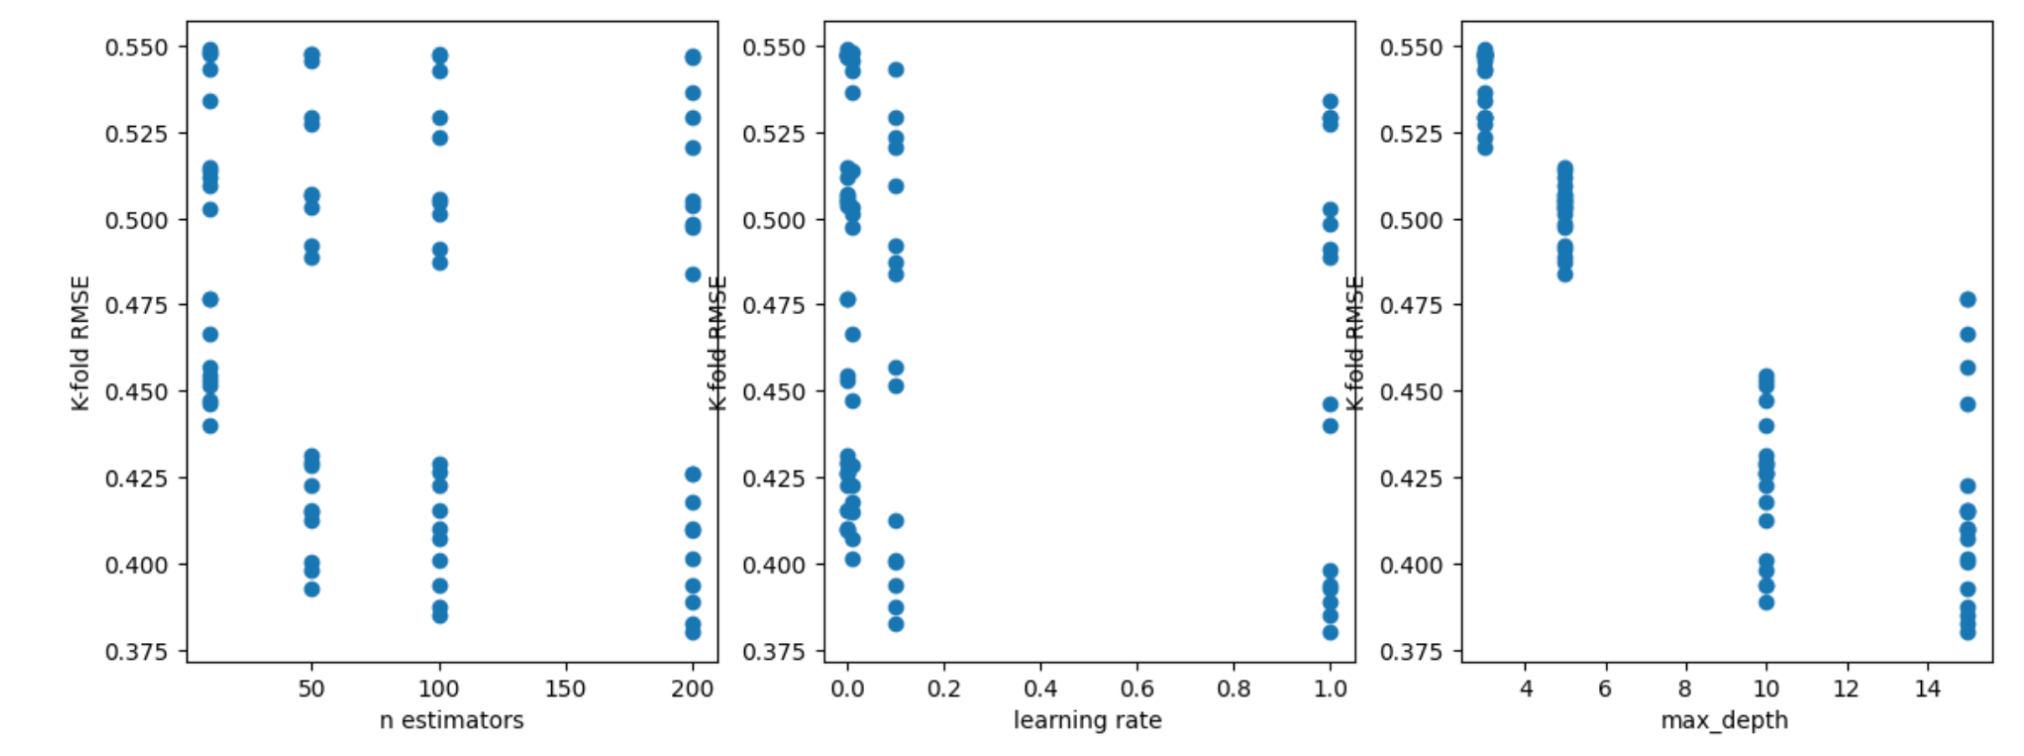
\includegraphics{Project_Report_Saturn_files/figure-pdf/ada1.png} Figure
1. 5 fold CV RMSE vs hyperparameters explored in the first GridSearchCV
for AdaBoost.

\begin{Shaded}
\begin{Highlighting}[]
\CommentTok{\# Second pass parameters considered}
\NormalTok{grid[}\StringTok{\textquotesingle{}n\_estimators\textquotesingle{}}\NormalTok{] }\OperatorTok{=}\NormalTok{ [}\DecValTok{200}\NormalTok{, }\DecValTok{500}\NormalTok{, }\DecValTok{1000}\NormalTok{]}
\NormalTok{grid[}\StringTok{\textquotesingle{}learning\_rate\textquotesingle{}}\NormalTok{] }\OperatorTok{=}\NormalTok{ [}\FloatTok{.5}\NormalTok{, }\FloatTok{.75}\NormalTok{, }\FloatTok{1.0}\NormalTok{]}
\NormalTok{grid[}\StringTok{\textquotesingle{}base\_estimator\_\_max\_depth\textquotesingle{}}\NormalTok{] }\OperatorTok{=}\NormalTok{ [}\DecValTok{12}\NormalTok{,}\DecValTok{14}\NormalTok{,}\DecValTok{16}\NormalTok{]}
\end{Highlighting}
\end{Shaded}

\begin{figure}

{\centering 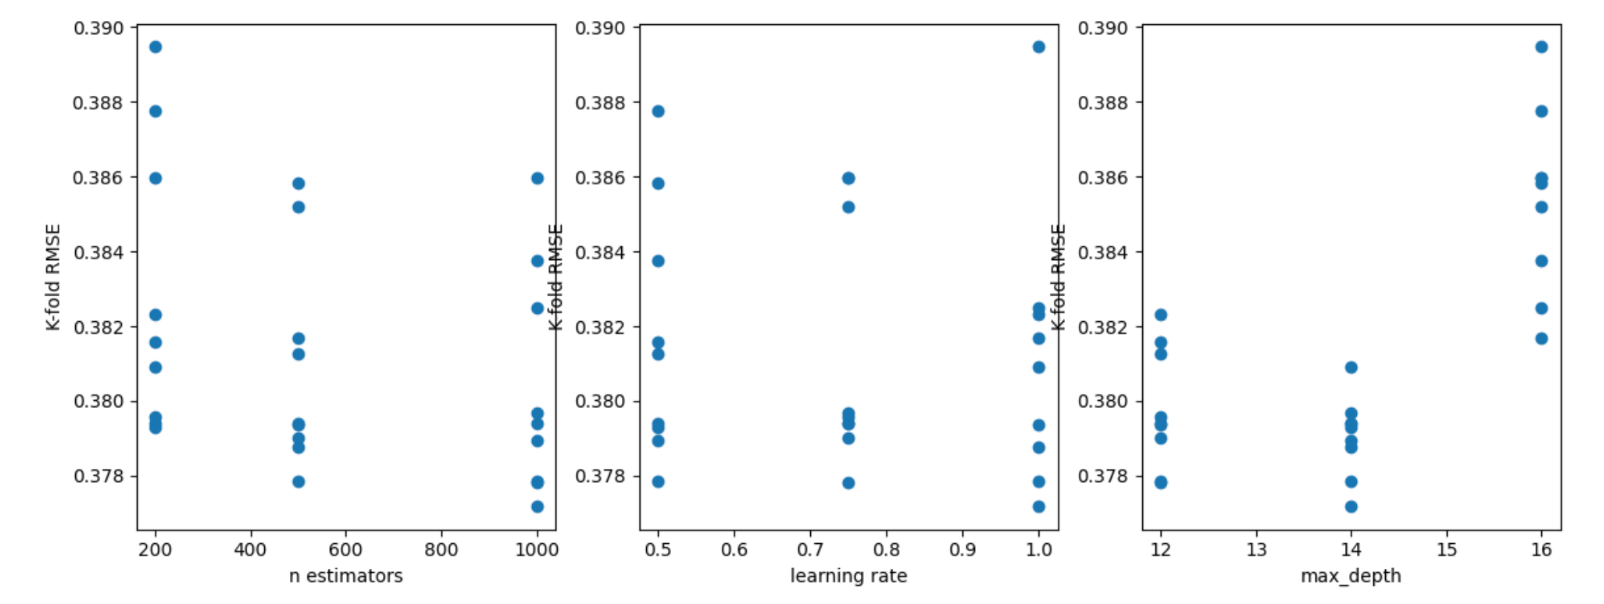
\includegraphics{Project_Report_Saturn_files/figure-pdf/ada2.png}

}

\caption{ada2.png}

\end{figure}

This gave the optimal hyperparameter values to be a \texttt{max\_depth}
of 14, \texttt{learning\_rate} as 1.0, and \texttt{n\_estimators} as
1000. I continued to narrow in to the optimal values with a finer grid
search.

\begin{Shaded}
\begin{Highlighting}[]
\CommentTok{\# Finer grid search parameters considered}
\NormalTok{grid[}\StringTok{\textquotesingle{}n\_estimators\textquotesingle{}}\NormalTok{] }\OperatorTok{=}\NormalTok{ [}\DecValTok{800}\NormalTok{, }\DecValTok{1000}\NormalTok{, }\DecValTok{1200}\NormalTok{, }\DecValTok{1500}\NormalTok{]}
\NormalTok{grid[}\StringTok{\textquotesingle{}learning\_rate\textquotesingle{}}\NormalTok{] }\OperatorTok{=}\NormalTok{ [}\FloatTok{.75}\NormalTok{, }\FloatTok{1.0}\NormalTok{, }\FloatTok{1.5}\NormalTok{]}
\NormalTok{grid[}\StringTok{\textquotesingle{}base\_estimator\_\_max\_depth\textquotesingle{}}\NormalTok{] }\OperatorTok{=}\NormalTok{ [}\DecValTok{13}\NormalTok{, }\DecValTok{14}\NormalTok{,}\DecValTok{15}\NormalTok{, }\DecValTok{16}\NormalTok{]}
\end{Highlighting}
\end{Shaded}

\begin{figure}

{\centering 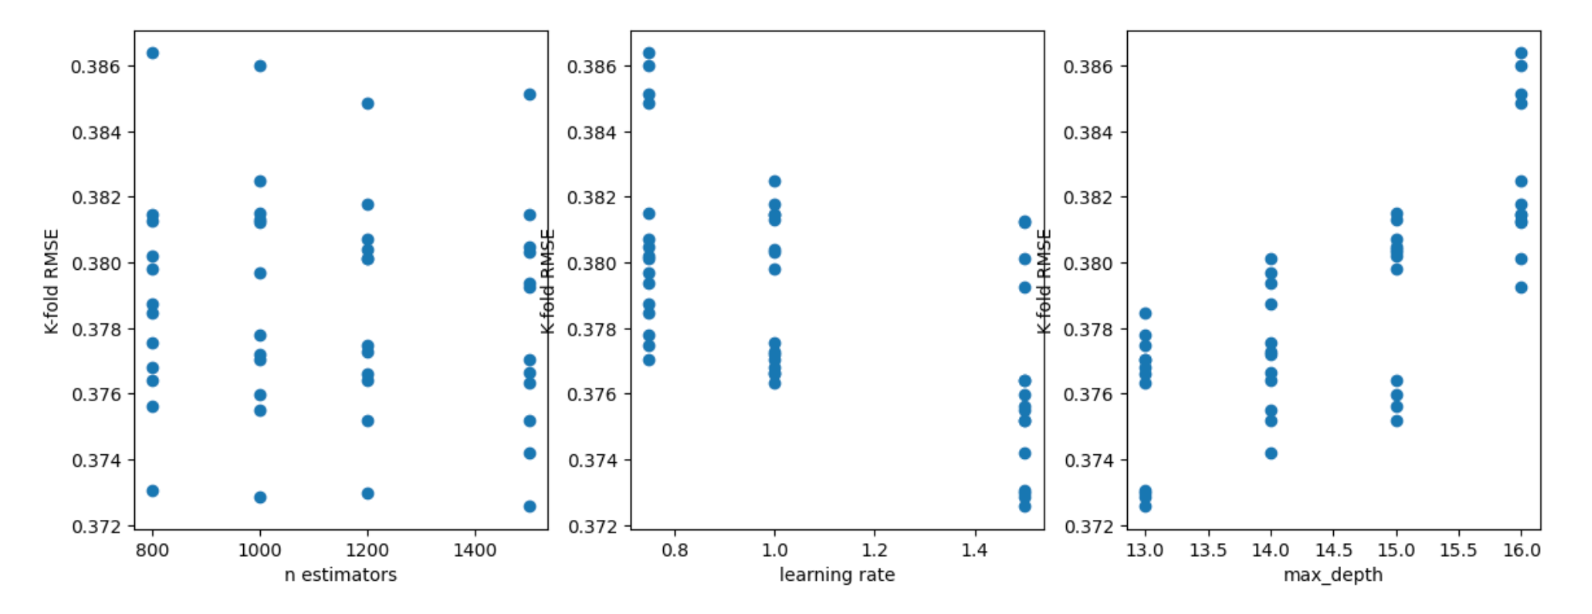
\includegraphics{Project_Report_Saturn_files/figure-pdf/ada3.png}

}

\caption{ada3.png}

\end{figure}

This gave the optimal values to be a \texttt{max\_depth} of 13,
\texttt{learning\_rate} of 1.5, and \texttt{n\_estimators} as 1500. As
some of these values are at the end of the range, I increased the values
I considered. I tuned \texttt{max\_depth} and \texttt{learning\_rate}
separately from \texttt{n\_estimators} as thus far, the highest value of
\texttt{n\_estimators} has been best.

\hypertarget{a5.-gradient-boosting}{%
\subsubsection{A5. Gradient Boosting}\label{a5.-gradient-boosting}}

\hypertarget{a6.-xgboost}{%
\subsubsection{A6. XGBoost}\label{a6.-xgboost}}

Figure 1: 5-fold cross-validated RMSE vs.~each parameter explored in the
first RandomizedSearchCV for XGBoost.

Method 1: Bayesian Optimization

With the following bounds, I conduct three Bayesian Optimization
searches:

\begin{quote}
pbounds = \{ `learning\_rate': (0.001, 1.0), `n\_estimators': (100,
4000), `max\_depth': (3,10), `subsample': (0.3, 1.0), `gamma': (0, 10),
`reg\_lambda': (0, 100)\}
\end{quote}

With 10 iterations and 5 initial points, I get the optimal combination:
\texttt{\{\textquotesingle{}colsample\textquotesingle{}:\ 0.926371203066647,\ \textquotesingle{}gamma\textquotesingle{}:\ 4.004543074048512,\ \textquotesingle{}learning\_rate\textquotesingle{}:\ 0.105068050089807,\ \textquotesingle{}max\_depth\textquotesingle{}:\ 6.815443879731223,\ \textquotesingle{}n\_estimators\textquotesingle{}:\ 1315.404330702919,\ \textquotesingle{}subsample\textquotesingle{}:\ 0.4879450393211324\}}.
A model trained with these parameters gave a higher RMSE of 0.7390, so I
decided to move forward with my best result from the RandomizedSearchCV
results.



\end{document}
